        %%******************************************%%
        %%                                          %%
        %%        Modello di tesi di laurea         %%
        %%            di Andrea Giraldin            %%
        %%                                          %%
        %%             2 novembre 2012              %%
        %%                                          %%
        %%******************************************%%


% I seguenti commenXeLaTeXti speciali impostano:
% 1. 
% 2. PDFLaTeX come motore di composizione;
% 3. tesi.tex come documento principale;
% 4. il controllo ortografico italiano per l'editor.

% !TEX encoding = UTF-8
% !TEX TS-program = pdflatex
% !TEX root = tesi.tex
% !TEX spellcheck = it-IT

\documentclass[12pt,                    % corpo del font principale
               a4paper,                 % carta A4
               oneside,                 % impagina per fronte-retro
               openright,               % inizio capitoli a destra
               english,                 
               italian,                 
               ]{memoir}    

%**************************************************************
% Importazione package
%************************************************************** 

%\usepackage{amsmath,amssymb,amsthm}    % matematica

\usepackage[T1]{fontenc}                % codifica dei font:
                                        % NOTA BENE! richiede una distribuzione *completa* di LaTeX

\usepackage{times}
\usepackage[headsep=.5in,left=1.5in,right=1.5in,top=1in,bottom=1in,footskip=.5in]{geometry}

\usepackage[utf8]{inputenc}             % codifica di input; anche [latin1] va bene
                                        % NOTA BENE! va accordata con le preferenze dell'editor

\usepackage[english, italian]{babel}    % per scrivere in italiano e in inglese;
                                        % l'ultima lingua (l'italiano) risulta predefinita

\usepackage{bookmark}                   % segnalibri

\usepackage{caption}                    % didascalie

\usepackage{chngpage,calc}              % centra il frontespizio

\usepackage{csquotes}                   % gestisce automaticamente i caratteri (")

\usepackage{emptypage}                  % pagine vuote senza testatina e piede di pagina
\usepackage{afterpage}                  % inserimento di pagine vuote

\usepackage{epigraph}			% per epigrafi

\usepackage{eurosym}                    % simbolo dell'euro

%\usepackage{indentfirst}               % rientra il primo paragrafo di ogni sezione

\usepackage{graphicx}                   % immagini

\usepackage{hyperref}                   % collegamenti ipertestuali

\usepackage[binding=5mm]{layaureo}      % margini ottimizzati per l'A4; rilegatura di 5 mm

\usepackage{listings}                   % codici

\usepackage{microtype}                  % microtipografia

\usepackage{mparhack,fixltx2e,relsize}  % finezze tipografiche

\usepackage{nameref}                    % visualizza nome dei riferimenti                                      

\usepackage[font=small]{quoting}        % citazioni

\usepackage{subfig}                     % sottofigure, sottotabelle

\usepackage[italian]{varioref}          % riferimenti completi della pagina

\usepackage[dvipsnames]{xcolor}         % colori

\usepackage{booktabs}                   % tabelle                                       
\usepackage{tabularx}                   % tabelle di larghezza prefissata                                    
\usepackage{longtable}                  % tabelle su più pagine                                        
\usepackage{ltxtable}                   % tabelle su più pagine e adattabili in larghezza
\usepackage{float}                      % evitare che le tabelle cambino posizione
\renewcommand{\arraystretch}{2}         % Righe più alte nelle tabelle

\usepackage[toc, acronym]{glossaries}   % glossario
                                        % per includerlo nel documento bisogna:
                                        % 1. compilare una prima volta tesi.tex;
                                        % 2. eseguire: makeindex -s tesi.ist -t tesi.glg -o tesi.gls tesi.glo
                                        % 3. eseguire: makeindex -s tesi.ist -t tesi.alg -o tesi.acr tesi.acn
                                        % 4. compilare due volte tesi.tex.

\usepackage[backend=biber,style=verbose-ibid,hyperref,backref]{biblatex}
                                        % eccellente pacchetto per la bibliografia; 
                                        % produce uno stile di citazione autore-anno; 
                                        % lo stile "numeric-comp" produce riferimenti numerici
                                        % per includerlo nel documento bisogna:
                                        % 1. compilare una prima volta tesi.tex;
                                        % 2. eseguire: biber tesi
                                        % 3. compilare ancora tesi.tex.

\usepackage{kpfonts}

%**************************************************************
% Layout pagine
%**************************************************************

\setSingleSpace{1.1}
\SingleSpacing
\definecolor{chaptercolor}{gray}{0.8}
\newcommand\numlifter[1]{\raisebox{-2cm}[0pt][0pt]{\smash{#1}}}
\newcommand\numindent{\kern37pt}
\newlength\chaptertitleboxheight
\makechapterstyle{hansen}{
  \renewcommand\printchaptername{\raggedleft}
  \renewcommand\printchapternum{%
    \begingroup%
    \leavevmode%
    \chapnumfont%
    \strut%
    \numlifter{\thechapter}%
    \numindent%
\endgroup%
}
  \renewcommand*{\printchapternonum}{%
    \vphantom{\begingroup%
      \leavevmode%
      \chapnumfont%
      \numlifter{\vphantom{9}}%
      \numindent%
      \endgroup}
    \afterchapternum}
  \setlength\midchapskip{0pt}
  \setlength\beforechapskip{0.5\baselineskip}
  \setlength{\afterchapskip}{3\baselineskip}
  \renewcommand\chapnumfont{%
    \fontsize{4cm}{0cm}%
    \bfseries%
    \sffamily%
    \color{chaptercolor}%
  }
  \renewcommand\chaptitlefont{%
    \normalfont%
    \huge%
    \bfseries%
    \raggedleft%
  }%
  \settototalheight\chaptertitleboxheight{%
    \parbox{\textwidth}{\chaptitlefont \strut bg\\bg\strut}}
  \renewcommand\printchaptertitle[1]{%
    \parbox[t][\chaptertitleboxheight][t]{\textwidth}{%
      %\microtypesetup{protrusion=false}% add this if you use microtype
      \chaptitlefont\strut ##1\strut}%
}}
\chapterstyle{hansen}
\aliaspagestyle{chapter}{empty} % just to save some space

%**************************************************************
% file contenente le impostazioni della tesi
%**************************************************************

%**************************************************************
% Frontespizio
%**************************************************************

% Autore
\newcommand{\myName}{Giovanni Jiayi Hu}                                    
\newcommand{\myTitle}{Stato applicativo multi-finistra in JavaScript }

% Tipo di tesi                   
\newcommand{\myDegree}{Tesi di laurea triennale}

% Università             
\newcommand{\myUni}{Università degli Studi di Padova}

% Facoltà       
\newcommand{\myFaculty}{Corso di Laurea in Informatica}

% Dipartimento
\newcommand{\myDepartment}{Dipartimento di Matematica "Tullio Levi-Civita"}

% Titolo del relatore
\newcommand{\profTitle}{Prof.}

% Relatore
\newcommand{\myProf}{Gilberto Filè}

% Luogo
\newcommand{\myLocation}{Padova}

% Anno accademico
\newcommand{\myAA}{2017-2018}

% Data discussione
\newcommand{\myTime}{Settembre 2018}


%**************************************************************
% Impostazioni di impaginazione
% see: http://wwwcdf.pd.infn.it/AppuntiLinux/a2547.htm
%**************************************************************

\setlength{\parindent}{0pt}   % larghezza rientro della prima riga
\setlength{\parskip}{0pt}   % distanza tra i paragrafi


%**************************************************************
% Impostazioni di biblatex
%**************************************************************
\bibliography{bibliografia} % database di biblatex 

\defbibheading{bibliography} {
    \cleardoublepage
    \phantomsection 
    \addcontentsline{toc}{chapter}{\bibname}
    \chapter*{\bibname\markboth{\bibname}{\bibname}}
}

% \setlength\bibitemsep{1.5\itemsep} % spazio tra entry

\DeclareBibliographyCategory{opere}
\DeclareBibliographyCategory{web}

\addtocategory{opere}{womak:lean-thinking}
\addtocategory{web}{site:agile-manifesto}

\defbibheading{opere}{\section*{Riferimenti bibliografici}}
\defbibheading{web}{\section*{Siti Web consultati}}


%**************************************************************
% Impostazioni di caption
%**************************************************************
\captionsetup{
    tableposition=top,
    figureposition=bottom,
    font=small,
    format=hang,
    labelfont=bf
}

%**************************************************************
% Impostazioni di glossaries
%**************************************************************

%**************************************************************
% Acronimi
%**************************************************************
\renewcommand{\acronymname}{Acronimi e abbreviazioni}

\newacronym[description={\glslink{apig}{Application Program Interface}}]
    {api}{API}{Application Program Interface}

\newacronym[description={\glslink{umlg}{Unified Modeling Language}}]
    {uml}{UML}{Unified Modeling Language}

%**************************************************************
% Glossario
%**************************************************************
%\renewcommand{\glossaryname}{Glossario}

\newglossaryentry{apig}
{
    name=\glslink{api}{API},
    text=Application Program Interface,
    sort=api,
    description={in informatica con il termine \emph{Application Programming Interface API} (ing. interfaccia di programmazione di un'applicazione) si indica ogni insieme di procedure disponibili al programmatore, di solito raggruppate a formare un set di strumenti specifici per l'espletamento di un determinato compito all'interno di un certo programma. La finalità è ottenere un'astrazione, di solito tra l'hardware e il programmatore o tra software a basso e quello ad alto livello semplificando così il lavoro di programmazione}
}

\newglossaryentry{Cookies}
{
    name=\glslink{Cookies}{Cookies A},
    text=Cookies,
    sort=Cookies,
    description={Cookies}
}

\newglossaryentry{framework}
{
    name=\glslink{framework}{framework A},
    text=framework,
    sort=framework,
    description={framework}
}

\newglossaryentry{JavaScript}
{
    name=\glslink{JavaScript}{JavaScript A},
    text=JavaScript,
    sort=JavaScript,
    description={JavaScript}
}

\newglossaryentry{JSON}
{
    name=\glslink{JSON}{JSON A},
    text=JSON,
    sort=JSON,
    description={JSON}
}

\newglossaryentry{Pair Programming}
{
    name=\glslink{Pair Programming}{Pair Programming A},
    text=Pair Programming,
    sort=Pair Programming,
    description={Pair Programming}
}

\newglossaryentry{React}
{
    name=\glslink{React}{React A},
    text=React,
    sort=React,
    description={React}
}

\newglossaryentry{Redux}
{
    name=\glslink{Redux}{Redux A},
    text=Redux,
    sort=Redux,
    description={Redux}
}

\newglossaryentry{singleton}
{
    name=\glslink{singleton}{singleton A},
    text=singleton,
    sort=singleton,
    description={singleton}
}

\newglossaryentry{sprint}
{
    name=\glslink{sprint}{sprint A},
    text=sprint,
    sort=sprint,
    description={sprint}
}

\newglossaryentry{stand-up}
{
    name=\glslink{stand-up}{stand-up A},
    text=stand-up,
    sort=stand-up,
    description={stand-up}
}

\newglossaryentry{TypeScript}
{
    name=\glslink{TypeScript}{TypeScript A},
    text=TypeScript,
    sort=TypeScript,
    description={TypeScript}
}

\newglossaryentry{umlg}
{
    name=\glslink{uml}{UML},
    text=UML,
    sort=uml,
    description={in ingegneria del software \emph{UML, Unified Modeling Language} (ing. linguaggio di modellazione unificato) è un linguaggio di modellazione e specifica basato sul paradigma object-oriented. L'\emph{UML} svolge un'importantissima funzione di ``lingua franca'' nella comunità della progettazione e programmazione a oggetti. Gran parte della letteratura di settore usa tale linguaggio per descrivere soluzioni analitiche e progettuali in modo sintetico e comprensibile a un vasto pubblico}
}
 % database di termini
\makeglossaries


%**************************************************************
% Impostazioni di graphicx
%**************************************************************
\graphicspath{{immagini/}} % cartella dove sono riposte le immagini


%**************************************************************
% Impostazioni di hyperref
%**************************************************************
\hypersetup{
    %hyperfootnotes=false,
    %pdfpagelabels,
    %draft,	% = elimina tutti i link (utile per stampe in bianco e nero)
    colorlinks=true,
    linktocpage=true,
    pdfstartpage=1,
    pdfstartview=FitV,
    % decommenta la riga seguente per avere link in nero (per esempio per la stampa in bianco e nero)
    %colorlinks=false, linktocpage=false, pdfborder={0 0 0}, pdfstartpage=1, pdfstartview=FitV,
    breaklinks=true,
    pdfpagemode=UseNone,
    pageanchor=true,
    pdfpagemode=UseOutlines,
    plainpages=false,
    bookmarksnumbered,
    bookmarksopen=true,
    bookmarksopenlevel=1,
    hypertexnames=true,
    pdfhighlight=/O,
    %nesting=true,
    %frenchlinks,
    urlcolor=webbrown,
    linkcolor=RoyalBlue,
    citecolor=webgreen,
    %pagecolor=RoyalBlue,
    %urlcolor=Black, linkcolor=Black, citecolor=Black, %pagecolor=Black,
    pdftitle={\myTitle},
    pdfauthor={\textcopyright\ \myName, \myUni, \myFaculty},
    pdfsubject={},
    pdfkeywords={},
    pdfcreator={pdfLaTeX},
    pdfproducer={LaTeX}
}

%**************************************************************
% Impostazioni di itemize
%**************************************************************
\renewcommand{\labelitemi}{$\ast$}

%\renewcommand{\labelitemi}{$\bullet$}
%\renewcommand{\labelitemii}{$\cdot$}
%\renewcommand{\labelitemiii}{$\diamond$}
%\renewcommand{\labelitemiv}{$\ast$}


%**************************************************************
% Impostazioni di listings
%**************************************************************
\lstset{
    language=[LaTeX]Tex,%C++,
    keywordstyle=\color{RoyalBlue}, %\bfseries,
    basicstyle=\small\ttfamily,
    %identifierstyle=\color{NavyBlue},
    commentstyle=\color{Green}\ttfamily,
    stringstyle=\rmfamily,
    numbers=none, %left,%
    numberstyle=\scriptsize, %\tiny
    stepnumber=5,
    numbersep=8pt,
    showstringspaces=false,
    breaklines=true,
    frameround=ftff,
    frame=single
} 


%**************************************************************
% Impostazioni di xcolor
%**************************************************************
\definecolor{webgreen}{rgb}{0,.5,0}
\definecolor{webbrown}{rgb}{.6,0,0}


%**************************************************************
% Altro
%**************************************************************

\newcommand{\omissis}{[\dots\negthinspace]} % produce [...]

% eccezioni all'algoritmo di sillabazione
\hyphenation
{
    ma-cro-istru-zio-ne
    gi-ral-din
}

\newcommand{\sectionname}{sezione}
\addto\captionsitalian{\renewcommand{\figurename}{Figura}
                       \renewcommand{\tablename}{Tabella}}

\newcommand{\glsfirstoccur}{\ap{{[g]}}}

\newcommand{\intro}[1]{\emph{\textsf{#1}}}

%**************************************************************
% Environment per ``rischi''
%**************************************************************
\newcounter{riskcounter}                % define a counter
\setcounter{riskcounter}{0}             % set the counter to some initial value

%%%% Parameters
% #1: Title
\newenvironment{risk}[1]{
    \refstepcounter{riskcounter}        % increment counter
    \par \noindent                      % start new paragraph
    \textbf{\arabic{riskcounter}. #1}   % display the title before the 
                                        % content of the environment is displayed 
}{
    \par\medskip
}

\newcommand{\riskname}{Rischio}

\newcommand{\riskdescription}[1]{\textbf{\\Descrizione:} #1.}

\newcommand{\risksolution}[1]{\textbf{\\Soluzione:} #1.}

%**************************************************************
% Environment per ``use case''
%**************************************************************
\newcounter{usecasecounter}             % define a counter
\setcounter{usecasecounter}{0}          % set the counter to some initial value

%%%% Parameters
% #1: ID
% #2: Nome
\newenvironment{usecase}[2]{
    \renewcommand{\theusecasecounter}{\usecasename #1}  % this is where the display of 
                                                        % the counter is overwritten/modified
    \refstepcounter{usecasecounter}             % increment counter
    \vspace{10pt}
    \par \noindent                              % start new paragraph
    {\large \textbf{\usecasename #1: #2}}       % display the title before the 
                                                % content of the environment is displayed 
    \medskip
}{
    \medskip
}

\newcommand{\usecasename}{UC}

\newcommand{\usecaseactors}[1]{\textbf{\\Attori Principali:} #1. \vspace{4pt}}
\newcommand{\usecasepre}[1]{\textbf{\\Precondizioni:} #1. \vspace{4pt}}
\newcommand{\usecasedesc}[1]{\textbf{\\Descrizione:} #1. \vspace{4pt}}
\newcommand{\usecasepost}[1]{\textbf{\\Postcondizioni:} #1. \vspace{4pt}}
\newcommand{\usecasealt}[1]{\textbf{\\Scenario Alternativo:} #1. \vspace{4pt}}

%**************************************************************
% Environment per ``namespace description''
%**************************************************************

\newenvironment{namespacedesc}{
    \vspace{10pt}
    \par \noindent                              % start new paragraph
    \begin{description} 
}{
    \end{description}
    \medskip
}

\newcommand{\classdesc}[2]{\item[\textbf{#1:}] #2}
                     % file con le impostazioni personali

\begin{document}
%**************************************************************
% Materiale iniziale
%**************************************************************
\frontmatter
% !TEX encoding = UTF-8
% !TEX TS-program = pdflatex
% !TEX root = ../tesi.tex

%**************************************************************
% Frontespizio 
%**************************************************************

\thispagestyle{empty}

\begin{center}

\begin{LARGE}
\textbf{\myUni}\\
\end{LARGE}

\vspace{10pt}

\begin{large}
\textsc{\myDepartment}\\
\end{large}

\vspace{10pt}

\begin{large}
\textsc{\myFaculty}\\
\end{large}

\vspace{30pt}
\begin{figure}[htbp]
\begin{center}
\includegraphics[height=6cm]{logo-unipd}
\end{center}
\end{figure}
\vspace{30pt} 

\begin{LARGE}
\begin{center}
\textbf{\myTitle}\\
\end{center}
\end{LARGE}

\vspace{10pt} 

\begin{large}
\textsl{\myDegree}\\
\end{large}

\vspace{40pt} 

\begin{large}
\begin{flushleft}
\textit{Relatore}\\ 
\vspace{5pt} 
\profTitle \myProf
\end{flushleft}

\vspace{0pt} 

\begin{flushright}
\textit{Laureando}\\ 
\vspace{5pt} 
\myName
\end{flushright}
\end{large}

\vspace{30pt}

\line(1, 0){338} \\
\begin{normalsize}
\textsc{Anno Accademico \myAA}
\end{normalsize}

\end{center}

\input{inizio-fine/colophon}
\blankpage
% !TEX encoding = UTF-8
% !TEX TS-program = pdflatex
% !TEX root = ../tesi.tex

%**************************************************************
% Dedica
%**************************************************************
\cleardoublepage
\phantomsection
\thispagestyle{empty}
\pdfbookmark{Dedica}{Dedica}

\vspace*{3cm}

\begin{center}
A rock pile ceases to be a rock pile the moment a single man contemplates it, bearing within him the image of a cathedral. \\ \medskip
--- Antoine de Saint-Exupéry, The Little Prince
\end{center}

% !TEX encoding = UTF-8
% !TEX TS-program = pdflatex
% !TEX root = ../tesi.tex

%**************************************************************
% Sommario
%**************************************************************
\cleardoublepage
\phantomsection
\pdfbookmark{Sommario}{Sommario}
\begingroup

\chapter*{Sommario}

Il presente documento è la relazione finale del lavoro svolto durante il periodo di stage del laureando Giovanni Jiayi Hu presso l'azienda WorkWave Italy Srl, della durata di 312 ore. \\

Lo scopo dello stage è stato l'esplorazione delle più recenti tecnologie web per la realizzazione di applicazioni web multi-finestra. A tale scopo è stato necessario eseguire un'attività di Ricerca \& Sviluppo (R\&D), testarne la loro maturità e integrare tali tecnologie nel prodotto \textbf{WorkWave Route Manager}. Quest'ultima applicazione offre ai propri clienti e permette di pianificare, dirigere, tracciare e analizzare le rotte dei propri veicoli in tempo reale. \\

Nello specifico, l'obiettivo principale è poter estrarre porzioni di interfaccia grafica dall'applicazione in una nuova pagina web autonoma, ma sincronizzata a livello di stato applicativo. L'integrazione ha avuto difatti lo scopo di permettere la visualizzazione della mappa Google Maps, ricca di rotte ed veicoli, su un monitor separato full-screen. \\

Lo sviluppo ha portato dunque alla nascita della libreria denominata \textbf{Stargate}, ispirato dall'ononima serie tv di fantascienza. \\

Sia \textit{Stargate} che \textit{Route Manager} sono basati su TypeScript, un linguaggio tipizzato che compila in JavaScript, ed utilizzano le librerie React 16 e Redux 4. Maggiori informazioni sulle tecnologie sono disponibili in Appendice §\ref{tecnologie} di questo documento.

%\vfill
%
%\selectlanguage{english}
%\pdfbookmark{Abstract}{Abstract}
%\chapter*{Abstract}
%
%\selectlanguage{italian}

\endgroup			

\vfill


\blankpage
% !TEX encoding = UTF-8
% !TEX TS-program = pdflatex
% !TEX root = ../tesi.tex

%**************************************************************
% Ringraziamenti
%**************************************************************
\cleardoublepage
\phantomsection
\pdfbookmark{Ringraziamenti}{ringraziamenti}


\bigskip

\begingroup
\let\clearpage\relax
\let\cleardoublepage\relax
\let\cleardoublepage\relax

\chapter*{Ringraziamenti}

\noindent \textit{Innanzitutto, vorrei esprimere la mia gratitudine al Prof. Gilberto Filè, relatore della mia tesi, per la disponibilità che mi ha offerto durante il periodo di stage e per i preziosi insegnamenti durante questi tre anni.}\\

\noindent \textit{Un ringraziamento speciale a Cesare d'Amico e a tutti i colleghi di WorkWave per la calorosa accoglienza fin dai primi giorni di stage. E naturalmente un sentito grazie a Matteo Ronchi, che ha saputo sempre guidarmi saggiamente durante questa esperienza e condividere pazientemente le sue preziose conoscenze.}\\

\noindent \textit{Vorrei inoltre dare un caloroso abbraccio ad Elisa per l'affetto e per avermi insegnato ad amare i dettagli della vita. Un sentito ringraziamento invece per tutti gli amici, sia di università che di vita, i quali mi hanno sopportato e tenuto compagnia in questo percorso.}\\

\noindent \textit{Desidero infine ringraziare con affetto i miei genitori per il costante sostegno ed incitamento nei miei progetti e nelle mie decisioni.}\\

\bigskip

\noindent\textit{\myLocation, \myTime}
\hfill \myName

\endgroup


\blankpage
\input{inizio-fine/indici}
\cleardoublepage

%**************************************************************
% Materiale principale
%**************************************************************
\mainmatter
% !TEX encoding = UTF-8
% !TEX TS-program = pdflatex
% !TEX root = ../tesi.tex

%**************************************************************
\chapter{L'azienda}
\label{cap:azienda}

\section{Descrizione}

WorkWave, una divisione di IFS, è una società americana fondata nel 1984 che fornisce soluzioni di Field Service Management e che connette ogni aspetto del business attraverso le sue piattaforme unificate e di facile uso. L'insieme delle soluzioni della compagnia permettono facilmente ai professionisti del settore di assegnare ed automatizzare attività di vendita e marketing, migliorando l'efficienza ed incrementando il monitoraggio sulle operazioni sul campo attraverso soluzioni mobile. \\

Le piattaforme di WorkWave forniscono ad oltre 8 mila clienti un livello senza precedenti di analisi del business, permettendolo loro di aumentare l'efficienza, il guadagno e garantendo un'eccezionale customer experience.

\begin{figure}[H] 
  \centering 
  
\includegraphics[]{workwave-logo} 
  \caption{Logo dell'azienda WorkWave}
\end{figure}

\section{Servizi offerti}

WorkWave aiuta aziende nel campo Field Service Management, oltre che industrie di trasporti e logistica, a mitigare gli aspetti dolorosi che incontrano ogni giorno. Consente loro infatti di salvare tempo, spese e migliorando il servizio agli utenti. \\

Per Field Service Management si intendono risorse impiegate per instradare verso i domicili dei clienti, quali localizzazione dei veicoli, gestione delle attività degli operatori, pianificazione ed impiego delle attività, garanzia della sicurezza dei conducenti ed integrazione di tali funzionalità con depositi, fatturazione ed altri servizi back-office. \\

WorkWave fornisce a tale scopo sia soluzioni per l'installazione e manutenzione hardware che servizi software per l'aiuto della gestione di tali attività. \\

La suite dei servizi software cloud, mobile e marketing permette a compagnie di ogni dimensione di facilmente stimare attività, pianificare ed dirigere operatori mobili con facilità. Di seguito si elencano i principali prodotti correlati all'attività di stage:

\begin{itemize}
  \item \textit{WorkWave Service}: è un servizio software che consente di velocemente schedulare rotte efficienti, visionare la produttività in tempo reale degli operatori, visualizzare stime e gestire pagamenti;
  \item \textbf{WorkWave Route Manager}: è un set di servizi per la gestione dei veicoli al fine di migliorare l'efficienza e la scalabilità attraverso pianificazione dinamica e miglioramenti intelligenti delle rotte. L'algoritmo proprietario del Route Manager garantisce che le migliori rotte per gli operatori siano usate per salvare tempo, costi e migliorare la soddisfazione dei clienti;
  \item \textit{WorkWave GPS}: fornisce un'intuitiva panoramica dei propri veicoli e delle propie risorse con un potente servizio GPS che cattura le azioni dell'operatore e le posizioni in tempo reale dei veicoli. Permette inoltre di migliorare la sicurezza dei guidatori, segnalare comportamenti errati e riportare incidenti.
\end{itemize}

\section{Route Manager}

\begin{figure}[h] 
  \centering 
  
\includegraphics[width=0.5\columnwidth]{workwave-route-manager-logo} 
  \caption{Logo WorkWave Route Manager}
\end{figure}

\textit{WorkWave Italy} è la sede centrale europea di WorkWave, dove sono concentrati gli sviluppi dell'algoritmo di routing e del prodotto Route Manager, contesto di sviluppo delle attività descritte in questo documento. \\

\textbf{WorkWave Route Manager} invece automatizza la pianificazione delle rotte per migliorare l'efficienza e la comunicazione tra l'amministrazione ed i guidatori dei veicoli, in maniera completamente customizzabile tramite le sue API. \\

\begin{figure}[H] 
  \centering 
  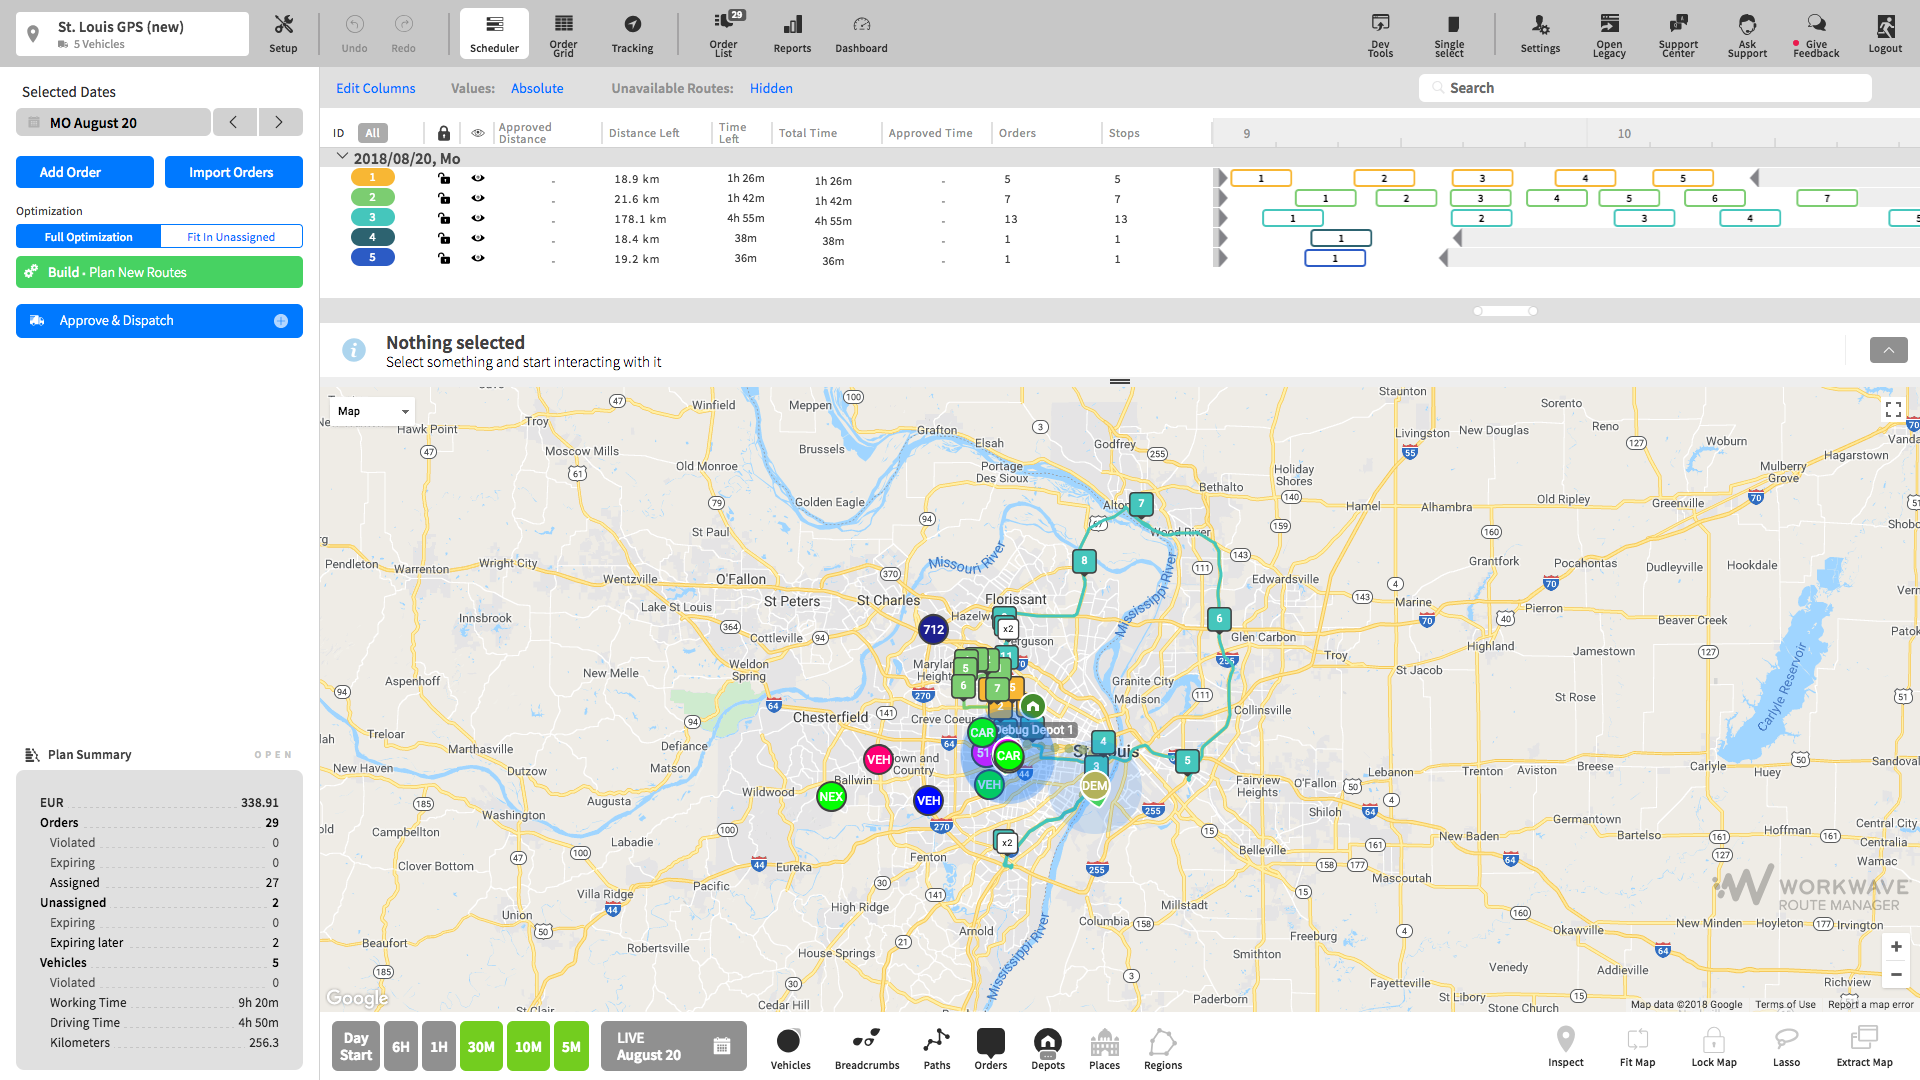
\includegraphics[width=1\columnwidth]{route-manager} 
  \caption{WorkWave Route Manager}
\end{figure}

In particolare, per quanto riguarda routing \& scheduling, rende possibile navigare attraverso gli orari di ricezione, schedulare le attività dei guidatori giornalmente ed eseguire report sulle performance. Attraverso le impostazioni, il software fornisce rotte ottimali in base ai propri vincoli stradali. \\

È inoltre possibile fare aggiustamenti manuali alle rotte via drag\&drop, approvare i piani e mandarli in esecuzione agli operatori sui veicoli. Oltre a ciò consente di visualizzare istantaneamente gli effetti delle modifiche sul numero di ordini possibili per i veicoli disponibili, il tempo stimato di completamento delle attività e comparare il costo per miglio.

\begin{figure}[H] 
  \centering 
  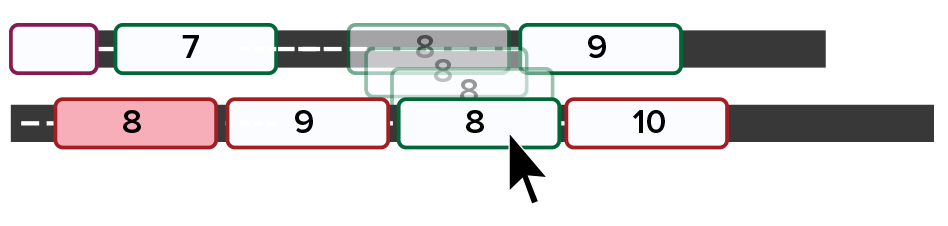
\includegraphics[width=1\columnwidth]{rm-scheduler} 
  \caption{WorkWave Route Manager - Scheduler degli ordini}
\end{figure}
             % Introduzione
% !TEX encoding = UTF-8
% !TEX TS-program = pdflatex
% !TEX root = ../tesi.tex

%**************************************************************
\chapter{Processi e metodologie}
\label{cap:processi-metodologie}
%**************************************************************

Durante il periodo di stage, ho avuto l'opportunità di entrare in contatto con i processi aziendali e diversi strumenti a supporto del mio lavoro, di seguito illustrati.

\section{Accertamento di Qualità}

Il processo di Accertamento di qualità provvede a garantire che il prodotto software sia conforme alle aspettative di qualità desiderate. Nello specifico, durante il mio periodo di stage, sono venuto a contatto con le seguenti pratiche di sviluppo.

\subsection{Pull Request}

\begin{figure}[H] 
  \centering 
  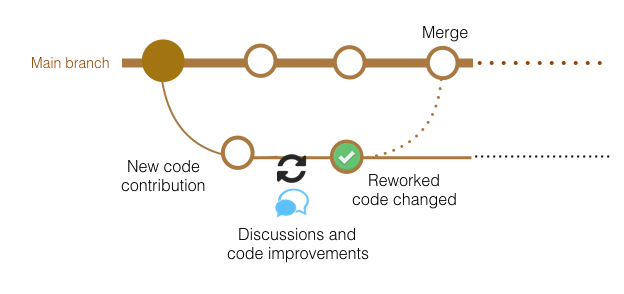
\includegraphics[width=0.75\columnwidth]{pull-request} 
  \caption{Flusso di una Pull Request}
\end{figure}

Una Pull Request è una proposta di modifica al repository effettuata su Github. Essa è obbligatoria per qualsiasi modifica e deve essere sempre realizzata tramite un git branch dedicato, avente un nome univoco e semantico rispetto alle modifiche proposte. \\

Lo scopo della Pull Request in WorkWave è favorire la discussione delle modifiche da parte del team e permetterne un'attenta ispezione prima ritenerla valida. Tuttavia essa è anche un'opportunità di apprendimento sia per chi esegue la review che per chi la riceve, in quanto entrambi hanno modo di apprendere diversi approcci allo stesso problema. \\

Essa permette anche, nel lungo termine, di venire a conoscenza di problematiche nel processo di sviluppo e poterle migliorare. Ad esempio la continua segnalazione di norme di sintassi è un indice della necessità di introdurre uno strumento automatico per la formattazione del codice.

\section{Gestione della configurazione}

\subsection{Versionamento}

L'azienda WorkWave organizza il proprio codice sorgente all'interno di diverse repository Git raggruppate sotto l'organizzazione GitHub dell'azienda. \\

In particolare è stato creato un repository dedicato al versionamento della prima fase della libreria \textit{Stargate} assieme al Proof of Concept. Successivamente il codice sorgente della libreria è stato direttamente integrato nel repository dell'applicazione \textit{Route Manager}.

\subsection{Ambiente di verifica}

\begin{figure}[H] 
  \centering 
  
\includegraphics[width=0.5\columnwidth]{jenkins} 
  \caption{Jenkins}
\end{figure}

Il processo di verifica è il più automatizzato possibile tramite tools eseguiti automaticamente con Jenkins \url{https://jenkins.io/}. Lo stesso procedimento avviene ad ogni Pull Request proibendone l’accettazione se le verifiche non sono superate.

Inoltre sono presenti script automatici che permettono di rilasciare in ambiente di sviluppo, demo, testing e produzione attraverso l'interfaccia grafica dashboard di Jenkins.

\subsection{Ambiente di rilascio}

\begin{figure}[H] 
  \centering 
  
\includegraphics[width=0.5\columnwidth]{clodfront} 
  \caption{Amazon Cloudfront}
\end{figure}

Il rilascio automatico eseguito da Jenkins porta al caricamento dell'applicazione \textit{Route Manager} su Amazon Cloudfront \url{https://aws.amazon.com/it/cloudfront/}, un servizio di Content Delivery Network (CDN) che permette di distribuire l'applicazione con latenza minima nei diversi Paesi del mondo.

\section{Gestione di Progetto}

\subsection{Standup}

Il team si incontra quotidianamente per lo standup, un incontro informale senza durata prefissata, che permette ai vari membri di allinearsi reciprocamente sullo stato di avanzamento ed eventuali problematiche. In particolare, nel caso di WorkWave tale attività è indispensabile in quanto vi sono alcuni del team che lavorano in remoto o negli Stati Uniti. \\

Tutti i membri, non solo i programmatori, sono invitati a partecipare e ad esporre su cosa stiano lavorando ed potenziali criticità, permettendo anche di trasmettere maggiore consapevolezza e conoscenza del progetto ai diversi partecipanti.

\subsection{Ticketing}

\begin{figure}[H] 
  \centering 
  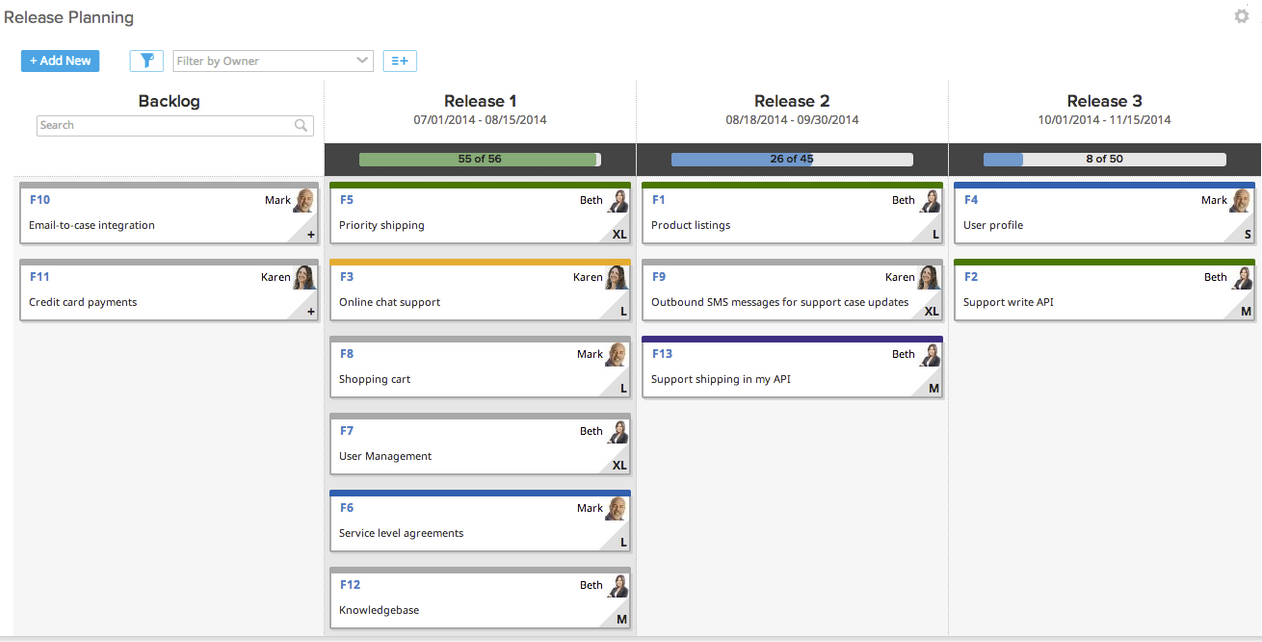
\includegraphics[width=1\columnwidth]{releaseplan_main} 
  \caption{CA Agile Central}
\end{figure}

L'azienda utilizza lo strumento CA Agile Central \footnote{ \url{https://www.ca.com/it/products/ca-agile-central.html}} per la gestione del ticketing, assegnando un ticket per ogni attività atomica. Ciò permette un'agevolazione nell'allineamento nel team sulle attività e gli obiettivi giorno per giorno. \\

Sono inoltre assegnate diverse priorità alle task al fine di garantire il completamento di quelle con maggior valore. Oltre a ciò è possibile avere un quadro complessivo del progresso, delle dipendenze e dell'allineamento della pianificazione durante ogni \gls{sprint}.
             % Stage
% !TEX encoding = UTF-8
% !TEX TS-program = pdflatex
% !TEX root = ../tesi.tex

%**************************************************************
\chapter{Processi e metodologie}
\label{cap:processi-metodologie}
%**************************************************************

Durante il periodo di stage, ho avuto l'opportunità di entrare in contatto con i processi aziendali e diversi strumenti a supporto del mio lavoro, di seguito illustrati.

\section{Accertamento di Qualità}

Il processo di Accertamento di qualità provvede a garantire che il prodotto software sia conforme alle aspettative di qualità desiderate. Nello specifico, durante il mio periodo di stage, sono venuto a contatto con le seguenti pratiche di sviluppo.

\subsection{Pull Request}

Una Pull Request è una proposta di modifica al repository effettuata su Github. Essa è obbligatoria per qualsiasi modifica e deve essere sempre realizzata tramite un git branch dedicato, avente un nome univoco e semantico rispetto alle modifiche proposte. \\

Lo scopo della Pull Request in WorkWave è favorire la discussione delle modifiche da parte del team e permetterne un'attenta ispezione prima ritenerla valida. Tuttavia essa è anche un'opportunità di apprendimento sia per chi esegue la review che per chi la riceve, in quanto entrambi hanno modo di apprendere diversi approcci allo stesso problema. \\

È stato inoltre spiegato che essa permette anche, nel lungo termine, di venire a conoscenza di problematiche nel processo di sviluppo e poterle migliorare. Ad esempio la continua segnalazione di norme di sintassi è un indice della necessità di introdurre uno strumento automatico per la formattazione del codice.

\section{Gestione della configurazione}

\subsection{Versionamento}

L'azienda WorkWave organizza il proprio codice sorgente all'interno di diverse repository Git raggruppate sotto l'organizzazione GitHub dell'azienda. In particolare è stato creato un repository dedicato al versionamento della prima versione della libreria \textit{Stargate} assieme al Proof of Concept. Successivamente il codice sorgente della libreria è stato direttamente integrato nel repository dell'applicazione \textit{Route Manager}.

\subsection{Ambiente di verifica}

\begin{figure}[H] 
  \centering 
  
\includegraphics[width=0.5\columnwidth]{jenkins} 
  \caption{Jenkins}
\end{figure}

Il processo di verifica è il più automatizzato possibile tramite tools eseguiti automaticamente con Jenkins \url{https://jenkins.io/}. Lo stesso procedimento avviene ad ogni Pull Request proibendone l’accettazione se le verifiche non sono superate.

Inoltre sono presenti script automatici che permettono di rilasciare in ambiente di sviluppo, demo, testing e produzione attraverso l'interfaccia grafica dashboard di Jenkins.

\subsection{Ambiente di rilascio}

\begin{figure}[H] 
  \centering 
  
\includegraphics[width=0.5\columnwidth]{clodfront} 
  \caption{Amazon Cloudfront}
\end{figure}

Il rilascio automatico eseguito da Jenkins porta al caricamento dell'applicazione \textit{Route Manager} su Amazon Cloudfront \url{https://aws.amazon.com/it/cloudfront/}, un servizio di Content Delivery Network (CDN) che permette di distribuire l'applicazione con latenza minima nelle diversi Paesi del mondo.

\section{Gestione di Progetto}

\subsection{Stand-up}

Il team si incontra quotidianamente per lo stand-up, un incontro informale senza durata prefissata, che permette ai vari membri di allinearsi reciprocamente sullo stato di avanzamento ed eventuali problematiche. In particolare, nel caso di WorkWave tale attività è indispensabile in quanto vi sono alcuni del team che lavorano in remoto o negli Stati Uniti.

Tutti i membri, non solo i programmatori, sono invitati a partecipare e ad esporre su cosa stiano lavorando ed potenziali criticità, permettendo anche di trasmettere maggiore consapevolezza e conoscenza del progetto ai diversi partecipanti.

\subsection{Ticketing}

\begin{figure}[H] 
  \centering 
  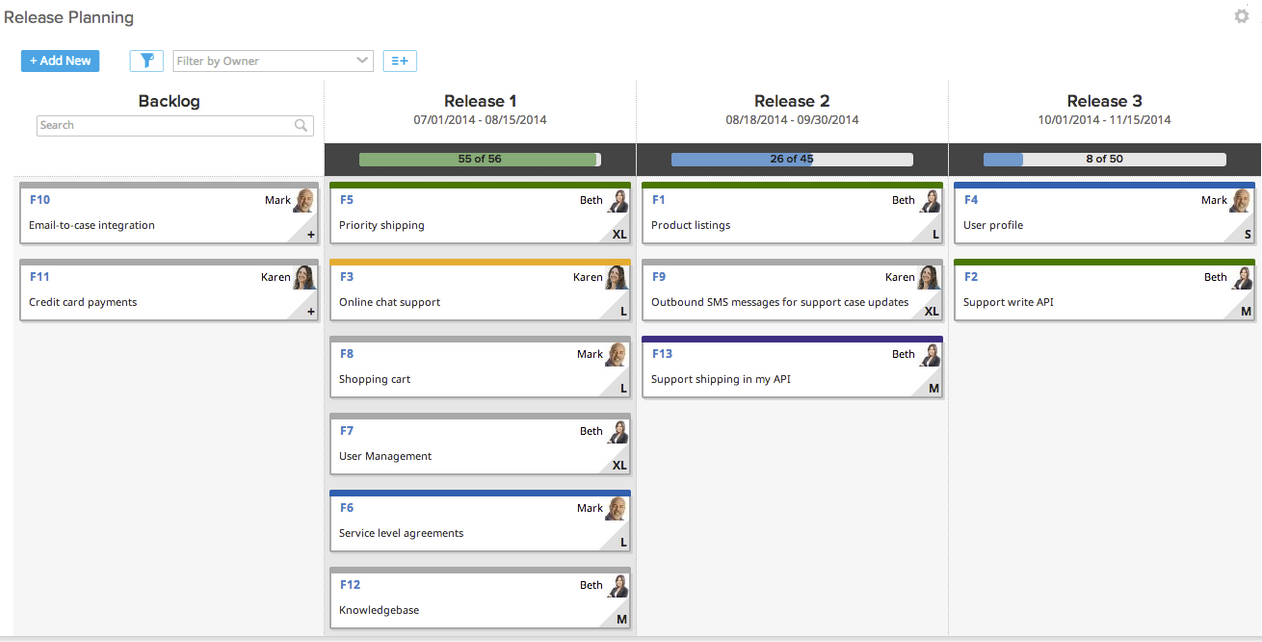
\includegraphics[width=1\columnwidth]{releaseplan_main} 
  \caption{CA Agile Central}
\end{figure}

L'azienda utilizza lo strumento CA Agile Central \url{https://www.ca.com/it/products/ca-agile-central.html} per la gestione delle attività.
             % Processi
\blankpage
% !TEX encoding = UTF-8
% !TEX TS-program = pdflatex
% !TEX root = ../tesi.tex

%**************************************************************
\chapter{Architettura per la comunicazione cross-page}
\label{cap:architettura}
%**************************************************************

In questo capitolo viene presentata prima l'architettura multi-process dei browser, in particolare di Chrome, per la gestione delle pagine web. Uno degli obiettivi è difatti la possibilità di eseguire i componenti nelle finestre figlie come processi separati, in modo da migliorare e non inficiare il processo dell'applicazione principale.

In seguito si illustra invece lo stato dell'arte delle diverse soluzioni per la comunicazione cross-page in JavaScript tra pagine su tab diverse. \\

Entrambe le sezioni fungono da spiegazione del contesto tecnologico in cui è stata sviluppata la soluzione \textit{Stargate} ed, al termine di esse, viene presentata una prima architettura naive per la libreria.

\section{Architettura multi-processi}

By design, JavaScript ha un modello di esecuzione single-threaded, ovvero tutte le sue istruzioni sono eseguite da un unico thread invece di averne diversi concorrenti. Ciò ha determinato la natura fortemente asincrona delle sue API, ove si cerca sempre di liberare il thread per i calcoli successivi appena possibile.

Qualora invece sia eccessivo il lavoro computazionale di una parte dell'applicazione, il risultato porta ad un'interfaccia bloccata e non responsiva fino al termine del calcolo. Questo ha un pessimo effetto sull'utente, in quanto l'applicazione non risponde alle sue interazioni e sembra anzi congelata. Per tale motivo è essenziale in primis che \textit{Stargate} esegua le nuove finestre su processi separati, al fine di non appesantire l'applicazione padre. \\

Quando la maggior parte dei browser moderni fu progettata inizialmente, le pagine web erano semplici e avevano poco o nessun codice attivo. Per tale motivo, i browser renderizzano tutte le pagine usando lo stesso processo, al fine di mantenere basso l'utilizzo delle risorse. \\

Tuttavia, le pagine web odierne sono decisamente più attive a partire da siti statici ma con tanto uso di JavaScript fino a vere e proprie applicazioni web come Gmail. Grosse parti di queste applicazioni girano all'interno del browser, così come le normali applicazioni eseguono in un sistema operativo e, proprio come questi, il browser deve dunque tenere le applicazioni separate tra di loro. \\

Oltre a ciò, le parti del browser che renderizzano HTML, JavaScript e CSS sono diventate straordinariamente complesse nel corso del tempo. Diventa perciò palese che browser i quali pongono tutto il lavoro in un processo affrontano seri problemi di rubustezza, responsitività e sicurezza. \\

Se un'applicazione web causasse un crash nel rendering engine, porterebbe la terminazione anche delle altre pagine web aperte. Le applicazioni web inoltre competono reciprocamente per l'uso della CPU ed ognuna di esse è single-thread per design di JavaScript, per cui rischierebbero di diventare non responsive alle interazioni utente. Infine anche la sicurezza è un fattore in rischio poiché una pagina web potrebbe sfruttare vulnerabilità del browser per accedere a dati delle altre pagine nello stesso processo.

\subsection{Cosa fa ogni processo?}

\begin{figure}[H] 
    \centering 
    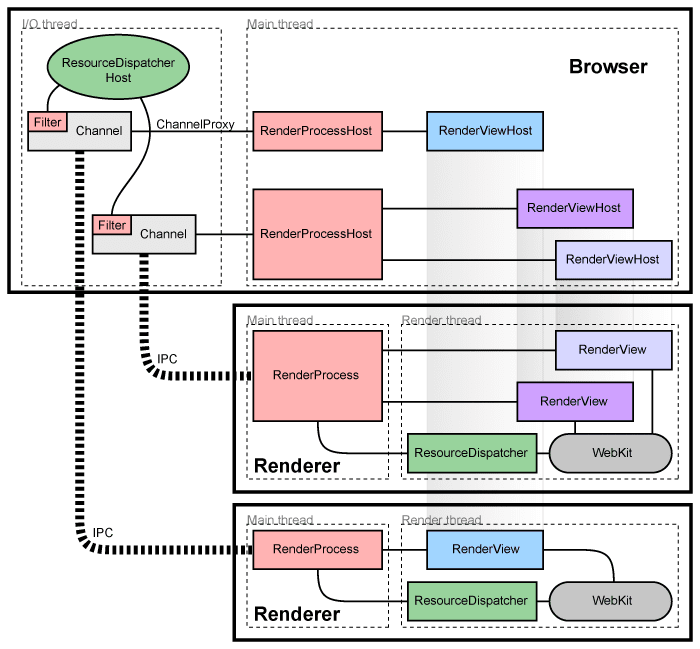
\includegraphics[width=1\columnwidth]{multi-process-arch} 
    \caption{Architettura multi-process in Chrome}
\end{figure}

Il browser crea tre differenti tipi di processi: browser, renderer ed estensioni.

\begin{itemize}
    \item \textbf{Browser}: esiste un unico processo browser, il quale gestisce i tab, le finestre e il browser stesso. Gestisce inoltre tutti i collegamenti delle pagine con il file system, la rete, input utente etc. ma non esegue alcun contenuto delle pagine;
    \item \textbf{Renderer}: il processo browser crea molteplici processi renderer, ognuno responsabile per la visualizzazione di una pagina web. I processi renderer contengono la complessa logica per la gestione di HTML, CSS, JavaScript, immagini e così via. Google Chrome, Safari ed altri utilizzano un rendering engine basato sul progetto open-source WebKit, mentre Firefox ed Edge hanno il proprio;
    \item \textbf{Estensioni}: il processo browser crea anche un processo per ogni estensione
\end{itemize}

\subsection{Strategie multi-process}

Una volta che il browser ha creato il processo omonimo, crea un processo renderer per ogni istanza di pagina web visitata dall'utente. Può essere pensato come un processo separato per ogni tab del browser, ma con l'eccezione di consentire a due tab di convidere lo stesso processo qualora siano collegati tra di loro e mostrino lo stesso sito. \\

Per esempio, se un tab ne apre un altro usando JavaScript o se viene aperto un link verso lo stesso sito in un nuovo tab, questi condivideranno lo stesso processo renderer. Si permette così ai tab correlati di comunicare via JavaScript e condividere la cache. Al contrario, se viene aperta una pagina di un sito diverso verrò riservato un nuovo processo. \\

Per essere precisi, si definisce un "sito" come un dominio registrato (ad esempio google.come o bbc.co.uk) e racchiude anche i sotto-domini (mail.google.com) e le porte (google.com:8080). Un' "istanza di sito" è invece un'insieme di pagine collegate provenienti dallo stesso sito. Due pagine sono considerate connesse se vi sono riferimenti reciproci in codice JavaScript, ad esempio una apre la seconda programmaticamente. Mentre se l'utente digita manualmente lo stesso indirizzo in due tab diverse, vengono considerate due istanze diverse con processi distinti. \\

Di seguito si illustrano nel dettaglio le diverse strategie multi-processi adottati dai browser moderni.

\subsubsection{Process-per-site-instance}

Normalmente i browser usano una strategia "Process-per-site-instance", ovvero lo stesso sito aperto in tab diversi con riferimenti reciproci saranno renderizzati dallo stesso processo. A volte è difatti necessario o desiderabile condividere il processo, quando per esempio un'applicazione web apre una nuova finestra con cui si aspetta di comunicare in maniera sincrona. \\

In generale invece, ogni nuova finestra o tab che non siano lo stesso sito possiede un nuovo processo.

\subsubsection{Process-per-site}

Raggruppa tutte le pagine dello stesso sito nello stesso processo, indipendentemente dalla presenza di riferimenti reciproci. Questa strategia è basata esclusivamente sul dominio del contenuto e non sulle relazioni tra le tab. Di conseguenza può risultare in processi molto onerosi.

\subsubsection{Process-per-tab}

Esiste anche una strategie più semplice che dedica un processo renderer per ogni gruppo di tab. Per ovvi motivi è estremamente inefficiente.

\subsection{Come forzare l'uso di un nuovo processo}

Dalla descrizione precedente della strategia \textit{Process-per-site-instance}, sembrerebbe non sia possibile ottenere l'effetto desiderato per il progetto \textit{Stargate}. Si desidera difatti alloccare un processo dedicato ad ogni finestra, sebbene appartengano allo stesso sito e quindi contrariamente al comportamento della strategia \textit{Process-per-site-instance}. \\

In seguito a diverse ricerche è tuttavia emerso che è possibile ottenere un processo dedicato come effetto collaterale di un parametro di sicurezza per la creazione delle nuove finestre. Nei browsers moderni è difatti possibile specificare un parametro \texttt{rel=noopener}, che evita exploits di sicurezza in cui la finestra padre è capace di accedere a riferimenti contenuti nella finestra figlia e/o viceversa. 

Quest'ultimo comportamento di condivisione dei riferimento è necessario per il corretto funzionamento di molte applicazioni cross-page, ma pone gli utenti a rischio qualora le nuove finestre siano di dominio diverso e potenzialmente maligne. Tramite il parametro \texttt{rel=noopener} è invece possibile evitare qualsiasi riferimento tra le parti e per, salvaguardare la sicurezza della memoria, ogni finestra creata con tale parametro ha un proprio processo dedicato. \\

Tramite quindi questa funzionalità, la libreria \textit{Stargate} è in grado di forzare un processo per ogni nuova finestra widget. L'altra faccia della medaglia, tuttavia, è la maggior difficoltà di comunicazione tra le finestre in quanto non si possiede più alcun riferimento JavaScript alle finestre. Per tale motivo si sono studiate diverse strategie di comunicazione cross-page, descritte nella prossima sezione.

\section{Comunicazione cross-page}

Nel corso degli anni vi sono state diverse strategie per la comunicazione cross-page tra pagine web in diversi tab, per soddisfare casi d'uso quali fare il check-out in una nuova pagina protetta di PayPal e notificare la pagina principale del risultato. Un altro esempio d'uso è la possibilità di avere una chat in una pagina separata, che tuttavia scambi informazioni con l'applicazione principale. Ed infine ovviamente il caso d'uso in questione, ovvero estrarre componenti UI per i monitor multipli. \\

\subsection{postMessage}

Il metodo \texttt{window.postMessage(message)} permette la comunicazione sicura attraverso istanze di finestre ed altri tipi di oggetti cross-page, ad esempio tra una pagina ed il popup che ha creato.

\texttt{targetWindow.postMessage(message);}

\begin{itemize}
    \item \textbf{targetWindow}: riferimento alla finestra che riceverà il messaggio. Alcuni esempi per ottenere tale riferimento sono:
        \begin{itemize}
            \item \texttt{window.open()} crea una nuova finestra;
            \item \texttt{window.opener} restituisce il riferimento alla finestra genitore che ha aperto la finestra corrente tramite il metodo precendete;
        \end{itemize}
    \item \textbf{message}: dati da inviare all'altra finestra. I dati sono serializzati usando lo \textit{structured clone algorithm} descritto successivamente, ma implica la possibilità di trasmettere una vasta varietà di oggetti in maniera safe senza doverli serializzare;
\end{itemize}

La finestra che riceve il messaggio può rimanere in ascolto attraverso la proprietà JavaScript \texttt{self.onmessage} che assegna alla propria pagina una funzione da invocare ogni volta che arriva un messaggio inviato da \textit{postMessage}.

\begin{lstlisting}
self.onmessage = function(message) {
    // Do something with message
}
\end{lstlisting}

\subsection{Eventi Storage}

Laddove l'API dedicata alla comunicazione cross-page \textit{postMessage} non si possa utilizzare, ad esempio su browsers meno moderni o perché non è possibile ottenere un riferimento alla finestra, è possibile usare gli eventi dello \texttt{Storage}. I browsers forniscono difatti delle API per la lettura e scrittura di dati persistenti anche dopo la chiusura della pagina. Inoltre lo storage è condiviso tra tutte le pagine aventi lo stesso dominio. \\

È quindi dunque possibile usare tali API per comunicare tra le finestre. \\

Esempio di invio di dati:

\begin{lstlisting}
// Salva nel proprio storage, che e' tuttavia condiviso tra 
// tab dello stesso dominio
window.localStorage.setItem('stargate-msg', message)
\end{lstlisting}

Esempio di ascolto di dati, ove si rimane in ascolto dell'evento di modifica dello Storage:

\begin{lstlisting}
window.addEventListener('storage', function(event) {
  const message = window.localStorage.getItem('stargate-msg')
})
\end{lstlisting}

È dunque palese che questo metodo sia un trick e non un'API nata allo scopo della comunicazione cross-page, tuttavia è stato utilizzato per anni anche a questo scopo. Un ulteriore aspetto inconveniente di questo approccio è il fatto che sia obbligatorio, a differenza di \textit{postMessage}, serializzare i dati in formato \gls{JSON}. Un confronto tra \textit{structured clone algorithm} e serializzazione è fornito in seguito in questo capitolo.

\subsection{Cookies}

È infine possibile utilizzare i cookies per la comunicazione tra finestre, laddove nemmeno gli eventi \texttt{Storage} siano possibili. La finestra che invia il messaggio lo serializza come stringa e lo scrive all'interno di un cookie del browser. La finestra ricevente è invece in ascolto tramite un timer che ogni tot millisecondi legge il cookie per capire se è stato cambiato. \\

Per diversi motivi quali limiti di dimensione dei cookie, difficoltà di lettura/scrittura, performance e scalabilità è una soluzione assolutamente sconsigliata. \\

Fortunatamente gli obiettivi obbligatori del progetto di stage richiedono il supporto solo di Google Chrome e Firefox, i quali supportano \textit{postMessage}. I browser invece supportati dal prodotto \textit{Route Manager}, ovvero fino ad Internet Explorer 11, supportano almeno gli eventi dello \texttt{Storage}, utilizzabili quindi come fallback.

\subsection{Structured clone algorithm VS Serialization}

Poiché la comunicazione è multi-finestra tra processi separati, è necessario purtroppo che i dati siano copiati da una finestra e l'altra per mantenersi sincronizzati. \\

Lo "Structured clone algorithm" è un algoritmo per la copia di oggetti JavaScript complessi ed è utilizzato internamento per il trasferimento di dati attraverso \textit{postMessage} ed altre API JavaScript. Ciò che fa è realizzare una copia analizzando ricorsivamente l'oggetto input, ma mantenendo una mappa dei riferimenti visitati precedentemente per evitare di attraversare infinitamente strutture circolari. 

Una struttura dati circolare consiste in un campo dell'oggetto il cui valore è il riferimento all'oggetto stesso in maniera diretta (\texttt{a -> a}) o indirettamente (\texttt{a -> b -> a}). \\

Vantaggi dello \textit{Structured clone algorithm}:

\begin{itemize}
    \item Supporto per strutture circolari;
    \item Supporto nativo per la copia di quasi qualsiasi tipo di oggetto JavaScript;
    \item Non vi è bisogno di convertire in un formato e ricostruire l'oggetto originale da tale formato, essendo quindi sia più performante che evitando di rischiare la perdita di informazioni durante la conversione.
\end{itemize}

Svantaggi dello \textit{Structured clone algorithm}:

\begin{itemize}
    \item Non è possibile clonare oggetti \texttt{Error} e \texttt{Function};
    \item Supportato dai browsers che supportano \textit{postMessage}
\end{itemize}

La serialization è invece una tecnica che consiste nel tradurre un oggetto JavaScript in un formato adatto per la trasmissione nelle rete o per il salvataggio. In JavaScript tale formato è una stringa JSON, comune anche ad altri linguaggi lato server.

Vantaggi della \textit{Serialization}:

\begin{itemize}
    \item Adatto per la trasmissione nella rete;
    \item Supportato da qualsiasi browser ed utilizza un formato comune ad altri linguaggi.
\end{itemize}

Svantaggi della \textit{Serialization}:

\begin{itemize}
    \item Non supporta strutture circolari di default;
    \item Supporta solo un sotto-insieme dei tipi di oggetti, in particolare solo i formati definiti dallo standard JSON: numeri, stringhe, booleani, oggetti letterali ed array. Non supporta ad esempio strutture dati quali \texttt{Map, Set, Date, ArrayBuffer}, etc.;
    \item Perdita di informazioni nella conversione oggetto <=> stringa JSON;
    \item Calcolo computazionale per conversione e ricostruzione dell'oggetto originale.
\end{itemize}

\subsection{Conclusioni}

Confrontando le diverse strategie per la comunicazione cross-page e la copia dei dati, è chiaro che la migliore sia l'utilizzo di \textit{postMessage}, il quale sfrutta lo \textit{Structured clone algorithm}. Difatti entrambi sono nati esattamente per uno scopo di comunicazione tra la pagina principale ed altre entità quali estensioni, altre finestre e Web Workers (spiegati in seguito).\\

È invece possibile utilizzare la tecnica degli \textit{Eventi Storage} assieme alla \textit{Serialization} come fallback della libreria \textit{Stargate} qualora il browser di esecuzione non supporti la strategia \textit{postMessage}. Tuttavia a causa delle nette differenze comportamentali tra \textit{Structured clone algorithm} e \textit{Serialization}, gli utilizzatori della libreria sono avvertiti delle possibili complicazioni. Posso quindi decidere se affidarsi al fallback, qualora non utilizzino alcuna struttura dati non supportata dalla \textit{Serialization}, oppure disabilitare l'utilizzo di \textit{Stargate} se il browser non è moderno.\\

Nel caso dell'azienda WorkWave per il prodotto \textit{Route Manager}, è stata decisa proprio la seconda opzione e disattivare l'interfaccia UI che permette di aprire la mappa Google Maps esternamente.

\section{Prima architettura Stargate}

Alla luce delle precedenti informazioni, si illustra di seguito una prima architettura per la libreria \textit{Stargate} e verrà ampliata passo per passo nei prossimi capitoli. Con la strategia \textit{postMessage} è difatti possibile organizzare l'applicazione nel seguente modo, ove si instraura una comunicazione bilaterale in cui \textit{Parent} trasferisce lo stato applicativo ed i vari \textit{Widget} notificano di eventi. \\

\begin{figure}[H] 
  \centering 
  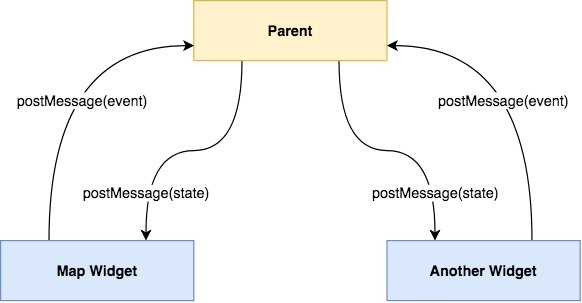
\includegraphics[width=1\columnwidth]{postMessage} 
  \caption{Prima architettura Stargate}
\end{figure}

\textbf{Parent}
    \begin{itemize}
        \item vive nella finestra principale ed è unica per sessione;
        \item si occupa della creazione e comunicazione con le finestre widget, mandando lo stato applicativo dell'applicazione contenente i dati necessari ai vari widget;
        \item gestisce gli eventi dei widget che necessitano di modificare lo stato applicativo dell'applicazione.
    \end{itemize}
\textbf{Widget}
    \begin{itemize}
        \item Vive in una finestra widget, creata dal \textit{Parent}
        \item Riceve lo stato applicativo ed utilizza i dati in essa per la corretta rappresentazione UI. Ogni volta che lo stato cambia, si aggiorna automaticamente anche la UI;
        \item Comunica al \textit{Parent} qualsiasi evento che abbia effetti sullo stato applicativo, ad esempio un'interazione utente.
    \end{itemize}
             % Architettura cross-page
% !TEX encoding = UTF-8
% !TEX TS-program = pdflatex
% !TEX root = ../tesi.tex

%**************************************************************
\chapter{Architettura per computazione parallela}
\label{cap:architettura-computazione-parallela}
%**************************************************************

La precedente architettura risponde all'esigenza di stabilire una comunicazione cross-page, ma lascia irrisolti diversi obiettivi del progetto. In questo capitolo viene invece presentata un'evoluzione di tale architettura, al fine di poter migliorare le performance di \textit{Stargate} ed offrire un sistema di gestione dei widget più indipendente.
Dal punto di vista delle performance, non è difatti sufficiente eseguire le nuove finestre in un processo separato. Sarebbe infatti più ottimale che il calcolo dello \textbf{stato derivato} venga effettuato una volta sola per tutti i widget della stessa tipologia.

\section{Stato derivato}

Per \textit{stato derivato} si intende l'insieme dei dati, calcolati a partire dallo stato applicativo dell'applicazione, necessari al widget per la corretta esecuzione di tutte le sue funzionalità. La funzione che calcola tali dati, avente per input lo stato applicativo e per output lo stato derivato, viene convenzionalmente denominata \textbf{selector} ed ha una firma di tipo \texttt{State => DerivedState}.

Tutte le funzioni \textit{selectors} devono inoltre essere pure \footnote{\url{https://en.wikipedia.org/wiki/Pure_function}}, ovvero ritornare lo stesso risultato a parità di input e non avere effetti collaterali (\textit{side-effects}), quali accesso/modifica a variabili non locali alla funzione, modifiche per riferimenti, accesso a I/O etc. \\

Nel seguente esempio lo stato applicativo rappresenta un'applicazione che gestisce una lista di acquisti. Si immagini quindi di avere un widget UI per mostrare il totale delle spese e che quindi necessiti di tale stato derivato.

\begin{lstlisting}[language={[Sharp]C}]
interface Purchase {
    name: number
    price: number
}

interface State {
    purchases: Array<Purchase>
}

type DerivedState = number

function sumSelector(state: State): DerivedState {
    let sum: number = 0;

    for (let i = 0; i < state.purchases.length; i++) {
        sum += state.purchases[i].price;
    }

    return sum
}
\end{lstlisting}

Essendo funzioni pure, è possibile comporre \textit{selectors} nella stessa maniera in cui si compongono funzioni matematiche \texttt{f ° g}, ottenendo \textit{selectors} più complessi ma comunque modulari. Il \textit{selector} finale di un componente UI può essere il risultato di decine di sotto-\textit{selectors}, a loro volte composti da altri \textit{selectors}.

\begin{figure}[H] 
  \centering 
  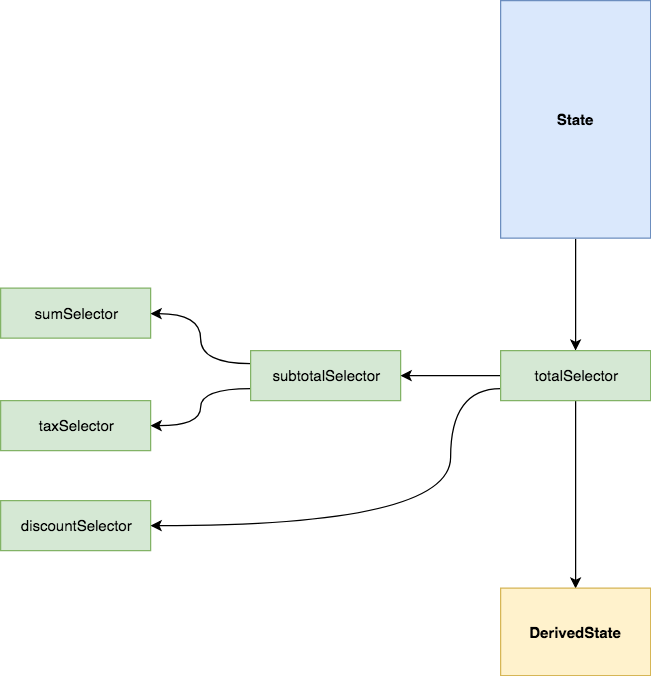
\includegraphics[width=1\columnwidth]{selectors} 
  \caption{Esempio di composizione di selectors}
\end{figure}

È facile quindi immaginare che in un componente UI complesso quale una mappa dei veicoli e rotte, tali \textit{selectors} siano molto complessi e richiedano un tempo di computazione non indifferente. \\

In particolare il codice JavaScript dell'applicazione principale è eseguito in un unico thread, per cui calcolare nell'applicazione padre lo stato derivato di diverse finestre con mappe potrebbe bloccare l'applicazione e renderla incapace di rispondere alle interazioni utenti fino al termine dei calcoli nei \textit{selectors}. \\

Una possibile soluzione potrebbe essere delegare tale calcolo nelle finestre figlie, poiché vivono su processi dedicati. Sebbene sia accettabile, non è ottimale in quanto il calcolo dei \textit{selectors} sarebbe ripetuto pur essendo identico per due finestre aventi entrambe la stessa tipologia di widget, per cui esiste un'alternativa migliore. \\

L'ideale è difatti calcolare lo stato derivato per ciascun tipo di widget una sola volta ad ogni modifica dello stato applicativo e propagare il risultato del calcolo ai widget, ad esempio a tutte le finestre contenenti la mappa. In tal modo l'onere computazionale è linearmente dipendente dal numero di \textbf{tipi di widget} attivi invece che dal numero totale di finestre. Tuttavia tale calcolo allo stesso tempo non può avere nella finestra padre per le stesse ragioni descritte sopra riguardo al eseguirlo in quelle figlie.

\section{Web Worker}\label{webworker}

\begin{figure}[H] 
  \centering 
  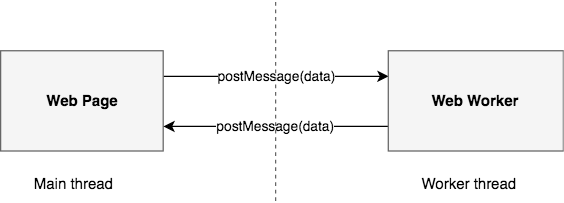
\includegraphics[width=1\columnwidth]{worker} 
  \caption{Comunicazione tra la pagine web ed il Web Worker}
\end{figure}

Un \textit{Web Worker} è un modo per una pagina web di eseguire del codice in un thread background, in grado di eseguire attività senza interferire con l'interfaccia utente. Nello specifico è un oggetto della classe \texttt{Worker}, creato passando come parametro il file che contiene il codice da eseguire nel thread separato. Tale thread non avrà alcun riferimento di memoria in comune con il main thread della pagina e viene considerato come un contesto di esecuzione separato. \\

È possibile eseguire qualsiasi tipo di codice all'interno del thread worker, con alcune eccezioni tuttavia. Ad esempio non è possibile manipolare direttamente i nodi HTML della pagina web o accedere ad API CSS/HTML. In generale un \textit{Web Worker} è da considerare un thread di calcolo computazione e non di manipolazione della pagina. \\

Un aspetto positivo è invece il sistema di comunicazione tra il worker and il thread principale dell'applicazione web, in quanto avviene anch'esso via \textit{postMessage} come se fosse tra finestre. Infine i \textit{Web Workers} possono attivare nuovi workers per delegare ulteriormente del lavoro in nuovi threads. \\

È quindi chiaro che un \textit{Web Worker} è il candidato ideale in \textit{Stargate} per l'esecuzioni dei \textit{selectors}. Nello specifico si desidera calcolare in un thread apposito lo stato derivato per ciascuna tipologia di widget, salvarla in cache ed inviarla a tutti i widget attivi di tale tipologia. Salvando in cache, è possibile renderizzare istantaneamente un widget alla sua apertura in quanto lo stato derivato necessario è stato già calcolato precedentemente.

Inoltre, poiché i calcoli avvengono in un thread di background, non vi sono impatti negativi nelle performance sia dell'applicazione principale che delle finestre widget. \\

Purtroppo l'utilizzo del \textit{Web Worker} genera un nuovo problema: le nuove finestre devono essere aperte comunque dalla pagina principale in quanto le relative API non sono disponibili nel Worker, ma non è quindi possibile per questi ottenerne i riferimenti per poter usare \texttt{widgetWindow.postMessage(derivedState)}. 

\section{BroadcastChannel}

Un \textit{BroadcastChannel} è un canale di comunicazione broadcast tra diversi "contesti" del browser (ad esempio finestre, tabs o workers) provenienti dallo stesso sito. È difatti disponibile anche da parte dei \textit{Web Workers}. \\

Creando un \textit{BroadcastChannel}, il quale rimane in ascolto del sottostante canale di comunicazione, si è in grado di inviare messaggi attraverso di esso usando \texttt{channel.postMessage(data)}, dunque usando il riferimento all'istanza di \textit{BroadcastChannel} invece che della finestra. Allo stesso tempo è possibile rimanere in ascolto di tutti i messaggi inviati attraverso il canale ed ogni messaggio è inviato a tutti coloro in ascolto, ovvero in broadcast. \\

È possibile quindi comunicare tra le parti senza riferimenti reciproci. Ogni parte dell'architettura è in grado di sottoscriversi al canale \textit{BroadcastChannel} ed avere una comunicazione bi-direzionale (\textit{full-duplex}) verso tutte le altre.

\begin{figure}[H] 
  \centering 
  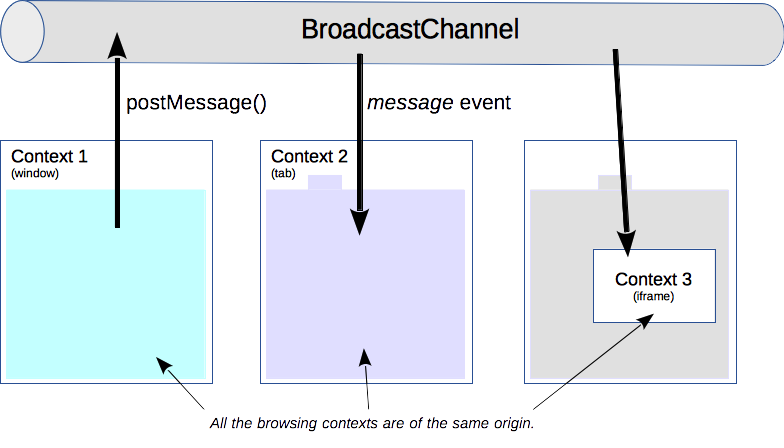
\includegraphics[width=1\columnwidth]{BroadcastChannel} 
  \caption{Esempio di funzionamento del BroadcastChannel}
\end{figure}

\section{Evoluzione architettura Stargate}

Alla luce degli aggiornamenti sui \textit{Web Workers} e sul \textit{BroadcastChannel}, si presenta la nuova architettura del progetto \textit{Stargate}.

\begin{figure}[H] 
  \centering 
  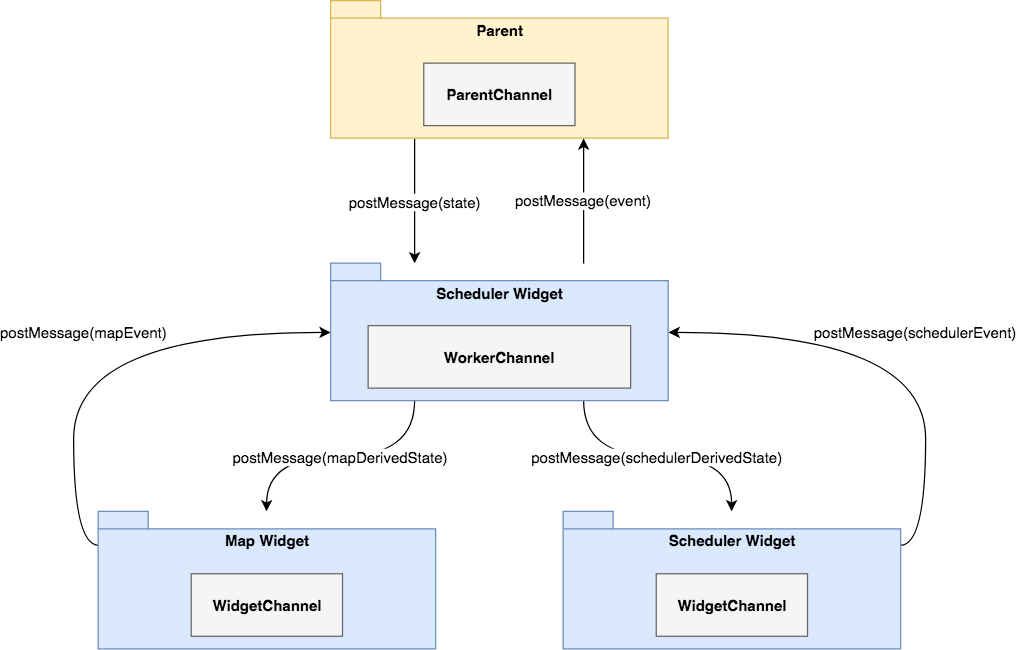
\includegraphics[width=1\columnwidth]{architettura2} 
  \caption{Architettura Stargate evoluta con Web Worker e BroadcastChannel}
\end{figure}

Le classi \textit{Parent} e \textit{Widget} sono divenute ora packages, in quanto contengono altre classi sottostanti tra cui quelle che gestiscono la comunicazione tramite \textit{BroadcastChannel}. \\

\textbf{ParentChannel}
    \begin{itemize}
        \item vive nella finestra principale ed è unica per sessione;
        \item gestisce il canale di comunicazione \textit{BroadcastChannel} verso il \textit{Web Worker};
        \item si occupa della creazione delle finestre widget, ma manda lo stato applicativo dell'applicazione al \textit{Web Worker} e \textbf{non} conosce le esigenze dei widget, a differenza all'architettura precedente;
        \item gestisce gli eventi dei widgets che necessitano di modificare lo stato applicativo dell'applicazione.
    \end{itemize}
\textbf{WorkerChannel}
    \begin{itemize}
        \item Vive nel \textit{Web Worker}, creato dal \textit{ParentChannel};
        \item Fa da intermediario per la comunicazione tra il \textit{ParentChannel} e tutti i diversi \textit{WidgetChannel};
        \item Riceve lo stato applicativo dal \textit{ParentChannel} e fornisce gli stati derivati a ciascun widget. Lo stato derivato, ad ogni modifica dello stato applicativo, è calcolato una volta sola per ogni tipologia di widget come descritto nelle sezioni precedenti;
        \item Propaga gli eventi dai \textit{WidgetChannel} verso il \textit{ParentChannel}.
    \end{itemize}
\textbf{WidgetChannel}
    \begin{itemize}
        \item Vive in una finestra widget, creata dal \textit{Parent};
        \item Riceve lo stato applicativo dal \textit{Web Worker} ed utilizza i dati in essa per la corretta rappresentazione UI. Ogni volta che lo stato cambia, si aggiorna automaticamente anche la UI;
        \item Comunica al \textit{Web Worker} (e non direttamente al \text{Parent}) qualsiasi evento che abbia effetti sullo stato applicativo, ad esempio un'interazione utente.
    \end{itemize}
             % Worker e BroadcastChannel
% !TEX encoding = UTF-8
% !TEX TS-program = pdflatex
% !TEX root = ../tesi.tex

%**************************************************************
\chapter{Diff \& patch}
\label{cap:diff-patch}
%**************************************************************

Uno degli obiettivi primari del progetto \textit{Stargate} è il supporto prestazionale a grosse mole di dati, dell'ordine di diversi MByte, in continuo aggiornamento ed uso. A questo punto del documento, l'architettura ottimizza il calcolo dello stato derivato attraverso i \textit{Web Workers} e tutte le operazioni dei widgets per via di un processo dedicato del Sistema Operativo. \\

Tuttavia entrambe le soluzioni non sono in grado di ottimizzare un potenziale collo-di-bottiglia delle performances: la trasmissione di grosse quantità di dati. Attualmente, ad ogni modifica dello stato applicativo, questi va inviato interamente al \textit{Web Worker} affinché possa calcolare gli stati derivati dei widgets, e tali stati sono a loro volta sono poi inviati ai widgets appunto. \\

Se da un lato tale scambio di dati non abbia impatti negativi sulla pagina principale grazie all'uso di \textit{Web Worker} e processi dedicati, dall'altro potrebbe causare un ritardo nei tempi di aggiornamento dell'Interfaccia Utente nelle finestre widget. Ciò causerebbe una cattiva percezione dell'utente nei confronti della fluidità d'uso dei componenti aperti nelle nuove finestre.

Un'interazione utente potrebbe richiedere un tempo sensibile per portare l'aggiornamento di tutte le finestre widget. \\

D'altra parte è inutilmente dispendioso il continuo invio di tutto lo stato applicativo, che deve essere copiato/serializzato da una parte all'altra. Per tale motivo è stato introdotto un sistema di \textit{diff \& patch} dello stato applicativo.

\section{Flusso diff \& patch}

\begin{enumerate}
  \item All'avvio dell'applicazione, viene inviato lo stato iniziale completo. Per completo si intende che non vi possono essere campi mancati rispetto alla sua interfaccia, sebbene possano avere come valore \texttt{null};
  \item Ad ogni successiva modifica dello stato applicativo, viene calcolata la differenza (ovvero il \textbf{delta $\Delta$}) tra il nuovo stato applicativo e quello precedente. Questa operazione viene chiamata \textbf{diffing};
  \item Il \textit{delta} contiene tutte le informazioni per ricostruire il nuovo stato a partire da quello vecchio. Tale \textit{delta} viene quindi inviato al \textit{Web Worker};
  \item Il \textit{Web Worker} applica il \textit{delta} sullo stato applicativo che ha in memoria, ottenendo il nuovo stato;
  \item Vengono ricalcolati gli stati derivati dei widgets ed un simile processo di \textit{diff \& patch} viene effettuato per essi. Difatti anche i widgets ricevono lo stato derivato intero solo alla loro apertura, ma i successivi aggiornamenti contengono solo i \textit{delta}.
\end{enumerate}

\begin{figure}[H] 
  \centering 
  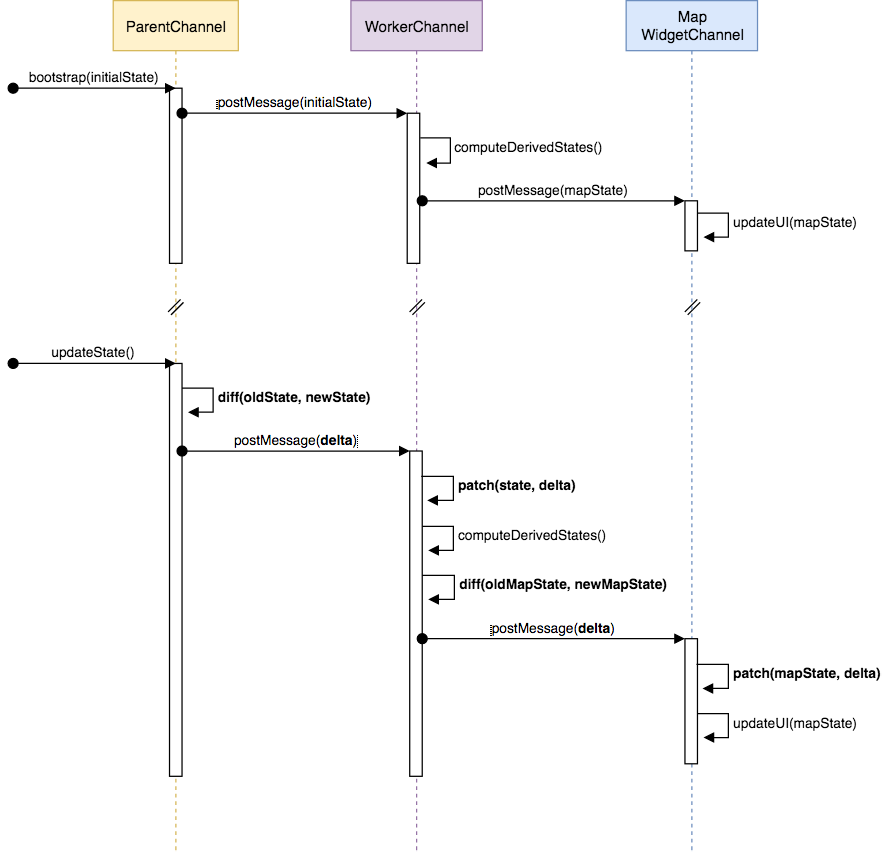
\includegraphics[width=1\columnwidth]{diff-patch} 
  \caption{Sequenza delle chiamate per il flusso diff \& patch}
\end{figure}

Si assicura in tal modo che le dimensioni del carico di trasmissione siano dipendenti unicamente dal numero di modifiche effettuate. Quest'ultime sono previste essere frequenti ma è ragionevole presupporre che ogni modifica statisticamente cambi solo una piccola porzione dello stato applicativo, risultando quindi in piccoli \textit{delta}. \\

\section{Ottimizzazione per immutable state}

Essendo inoltre \textit{Stargate} rivolto verso applicazioni web moderne, in particolare in React \& Redux, l'algoritmo interno di \textit{diff \& patch} assume anche che modifiche allo stato applicativo non vengano fatte per riferimento, ma bensì ritornino una copia aggiornata avente un nuovo riferimento e le cui proprietà siano anch'esse nuove laddove modificate. \\

Si parla nello specifico di \textit{strutture dati persistenti}.

\subsection{Strutture dati persistenti}

Una modifica per riferimento è una mutazione diretta ad una struttura dati esistente (un oggetto) senza crearne una copia. Una modifica \textbf{immutable} invece si assicura preventivamente di fare una copia, non profonda, dell'oggetto in qualsiasi caso in cui una proprietà cambi. \\

Ad esempio si assuma di voler modificare la proprietà \texttt{xs.d.g.f} sostituendo 1 con \texttt{\{ e: 1 \}}. 

\begin{lstlisting}[language={[Sharp]C},basicstyle=\footnotesize]
const xs = {
  d: {
    b: {
      a: 1,
      c: 1
    },
    g: {
      f: 1, // <== da sostituire con { e: 1 }
      h: 1
    }
  }
}
\end{lstlisting}

Modificarlo per riferimento sarebbe eseguire l'istruzione JavaScript \texttt{xs.d.g.f = \{ e: 1 \}}, in quanto viene modificato il campo annidato \texttt{f}, ma sia \texttt{xs} che i suoi sotto-oggetti \texttt{d, g, f} mantengono lo stesso riferimento rispetto a prima. \\

Una modifica immutabile invece ritorna un nuovo oggetto \texttt{ys}, ove sia \texttt{ys} che i suoi sotto-oggetti \texttt{d', g', f'} hanno nuovi riferimenti mentre \texttt{b} è rimasto invariato poiché non modificato.

\begin{lstlisting}[language={[Sharp]C},basicstyle=\footnotesize]
const ys = {        // <== nuovo riferimento ys
  d: {              // <== nuovo riferimento d'
    b: {
      a: 1,
      c: 1
    },
    g: {            // <== nuovo riferimento g'
      f: { e: 1 },  // <== nuovo riferimento f'
      h: 1
    }
  }
}
\end{lstlisting}

Una possibile rappresentazione della precedente modifica \textit{immutable} è il seguente albero, ove il nuovo oggetto \texttt{ys} possiede sia riferimenti a nuovi oggetti (\texttt{d', g', f'} sono stati modificati), che a vecchi (\texttt{b, c, h} sono invariati).

\begin{figure}[H] 
  \centering 
  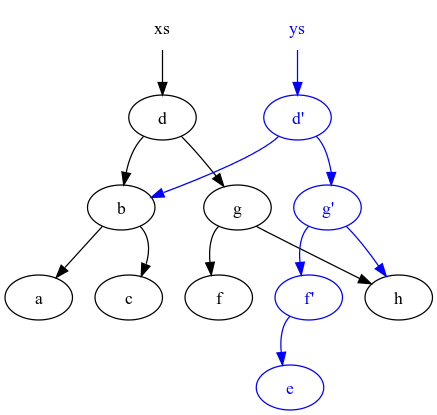
\includegraphics[width=0.5\columnwidth]{immutable} 
  \caption{Albero di \texttt{ys}, ove le parti blu hanno nuovi riferimenti}
\end{figure}

Strutture dati che preservano sempre la propria precedente versione in caso di modifica si chiamano \textbf{strutture dati persistenti} \footnote{\url{https://en.wikipedia.org/wiki/Persistent_data_structure}} e sono immutabili in quanto le loro operazioni non mutano direttamente la struttura, ma bensì generano sempre una nuova aggiornata. \\

Tali strutture dati sono fondamentali nei linguaggi di programmazione funzionali, ma nei recenti anni sono divenute fondamentali anche per linguaggi non puramente funzionali come JavaScript in quanto portano a diversi vantaggi come la diminuzione di \textit{side-effects}.

\subsection{Ottimizzazione dell'algoritmo}

Nel caso specifico dell'algoritmo \textit{diff \& patch}, le strutture immutabili permettono di ottimizzare il calcolo del \textit{delta} in quanto è sufficiente controllare per riferimento se un campo è cambiato rispetto a prima, senza dover controllare profondamente i valori. Ad esempio confrontando \texttt{xs} e \texttt{ys} dall'esempio precedente, l'algoritmo può evitare di proseguire il calcolo del \textit{delta} per l'intero sotto-albero \texttt{b} in quanto il riferimento non è cambiato. Se invece viene rilevato un diverso riferimento, l'algoritmo continua lavorando sul sotto-albero. \\

Per uno stato applicativo di notevoli dimensioni, questa ottimizzazione permette di migliorare notevolmente i tempi di \textit{diffing} dell'algoritmo, rendendo il costo linearmente dipendente al numero di modifiche invece che alle dimensioni della struttura.

Un controllo di riferimento per sapere se un sotto-albero è cambiato ha difatti tempo costante \texttt{O(1)}, altrimenti sarebbe direttamente proporzionale \texttt{$\Theta$(n)} al numero di campi annidati.
             % Product Design Freeze e SOP
% !TEX encoding = UTF-8
% !TEX TS-program = pdflatex
% !TEX root = ../tesi.tex

%**************************************************************
\chapter{Architettura per il Context}
\label{cap:architettura-context}
%**************************************************************

L'ultimo step di evoluzione del progetto \textit{Stargate} consiste nell'astrazione \textbf{da stato applicativo a Context}, ovvero contesto di esecuzione dei componenti UI. Sebbene difatti lo stato applicativo rappresenti nella maggioranza dei casi tutto ciò di cui un widget ha bisogno da parte dell'applicazione principale, in alcuni casi è necessario poter accedere anche ad altri oggetti ed addirittura richiamare metodi dalla finestra padre. \\

Si supponga difatti che il widget mappa utilizzi un'istanza \gls{singleton} della classe \texttt{GoogleMaps}, responsabile dei calcoli geografici attraverso le API di Google Maps e condivisa a molteplici componenti UI oltre alla mappa.

In questo caso, il widget mappa ha dunque bisogno del seguente "contesto" per poter correttamente funzionare anche al di fuori della pagina principale: \\

\begin{lstlisting}[language={[Sharp]C}]
interface MapContext {
  googleMaps: GoogleMaps
  state: State
}
\end{lstlisting}

Si può notare come il precedente stato applicativo \texttt{State}, sia ora una delle proprietà del \textit{Context} della mappa e sicuramente la più importante. Tuttavia il passaggio da stato applicativo ad un concetto più generale di "contesto", permette anche l'aggiunta all'interfaccia di un campo per l'istanza singleton di \texttt{GoogleMaps}, senza dover inserire questi nello stato applicativo di cui non fa parte logicamente. 

A livello di architettura fortunatamente vi è poco da modificare, in quanto si tratta solamente di ampliare il concetto di stato applicativo a \textit{Context} e quindi di rinominare i termini. Si parla quindi di \textbf{Context e DerivedContext} invece che \textit{State e DerivedState}.

\begin{figure}[H] 
  \centering 
  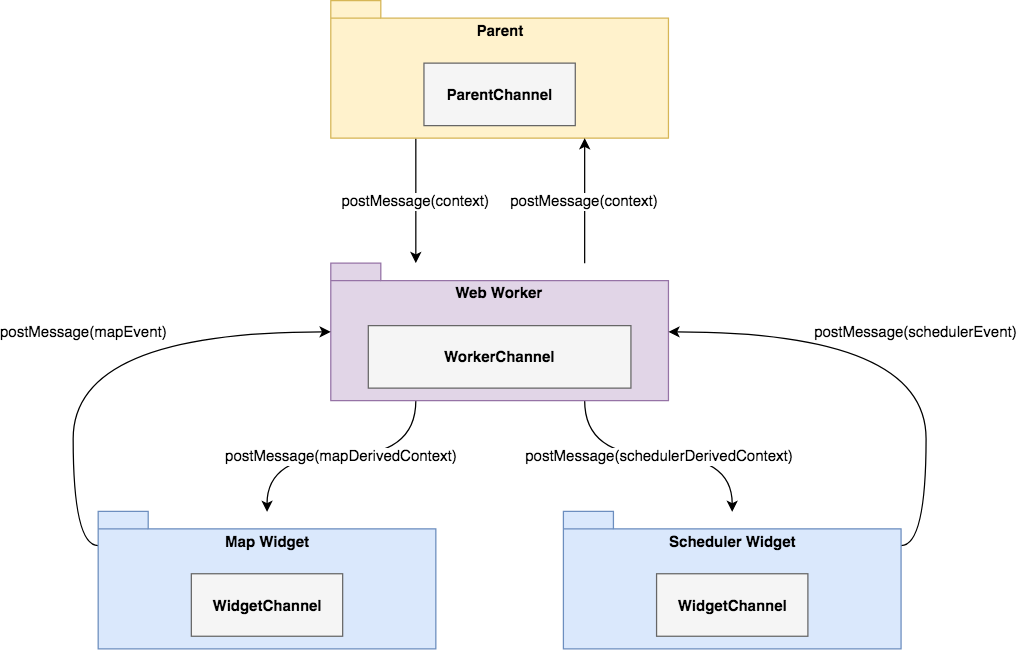
\includegraphics[width=1\columnwidth]{architettura3} 
  \caption{Architettura per il Context}
\end{figure}

\section{Remote Procedure Call (RPC)}

L'introduzione del \textit{Context} porta alla luce una nuova sfida: chiamate di metodi nella finestra padre da parte di widgets. Lo \textit{State} è infatti un'insieme di dati di sola lettura, ma l'istanza \texttt{GoogleMaps} viene invece utilizzata richiamandone metodi con passaggio di parametri e valori di ritorno attesi. \\

Tuttavia l'applicazione principale, il \textit{Web Worker} ed i widget non hanno alcuna condivisione di memoria per cui apparentemente sembrerebbe impossibile per una finestra figlia richiamare un metodo di un oggetto esistente solo nel padre. Nel caso di istanze singleton come \textit{GoogleMaps} non è possibile che ogni widget abbia la sua copia dell'oggetto, poiché violerebbe proprio la definizione di singleton. \\

In questi casi è necessario utilizzare \textbf{Remote Procedure Call (RPC)}, ovvero chiamate chiamate di procedure che avvengono in uno spazio di memoria diverso (solitamente un altro dispositivo della rete), ma in maniera trasparente come normali chiamate locali a procedure/metodi. È desiderabile infatti che il chiamante del \textit{metodo RPC} non conosca i dettagli implementativi della chiamata remota sottostante.

In Java vi è un'implementazione delle chiamate RPC attraverso le \textit{Remote method invocations (RMI)}. \\

Nel caso del progetto \textit{Stargate}, quando il widget esegue una chiamata di un metodo del \textit{Context}, ad esempio \texttt{context.googleMaps.getDistance(a, b)}, in realtà succede il seguente:

\begin{enumerate}
  \item Viene creato un messaggio contenente informazioni sulla chiamata, quali la proprietà del \textit{Context}, il nome del metodo ed i parametri;
  \item Il messaggio viene inviato al \textit{Web Worker};
  \item Il messaggio viene ritrasmesso al \textit{ParentChannel};
  \item Viene invocato l'effettivo metodo nella finestra padre, passando i parametri provenienti dal widget;
  \item Viene generato un messaggio contenente le informazioni della chiamata con l'eventuale valore di ritorno;
  \item Il messaggio di risposta viene inviato al \textit{Web Worker} e ritrasmesso al \textit{WidgetChannel};
  \item Il chiamante riceve il valore di ritorno e può proseguire con il resto della procedura
\end{enumerate}

Per ovvi motivi di performance, una volta chiamato il metodo, la finestra widget mette in pausa la procedura asincrona e prosegue con altre attività evitando di rimanere bloccata in attesa della risposta. L'inconveniente è difatti che tutte le chiamate di metodi nel \textit{Context} diventano asincrone, anche qualora fossero originariamente sincrone.

\begin{figure}[H] 
  \centering 
  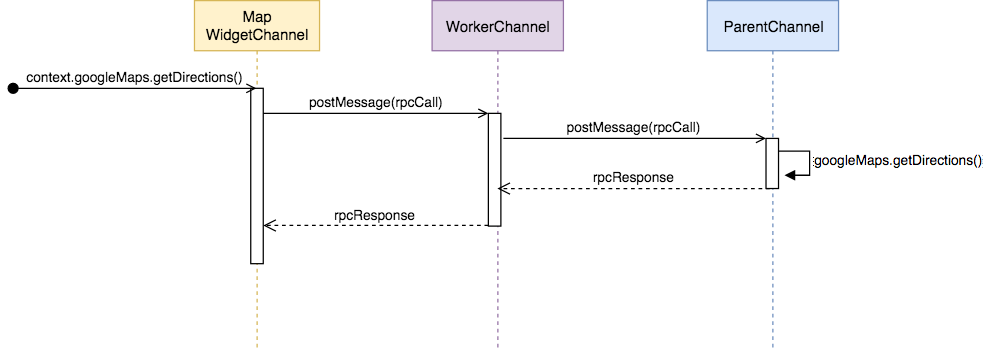
\includegraphics[width=1\columnwidth]{rpc} 
  \caption{Sequenza per una chiamata RPC del context}
\end{figure}


\subsection{Implementazione RPC tramite Proxy}

Ai fini di rendere la chiamata RPC trasparente nei confronti dell'utente, gli oggetti al primo livello di annidamento del \textit{Context} sono rimpiazzati da equivalenti \textit{Proxy}, che funzionano esattamente come gli originali ma racchiudono al loro interno la logica di comunicazione descritta poco prima.

\begin{figure}[H] 
  \centering 
  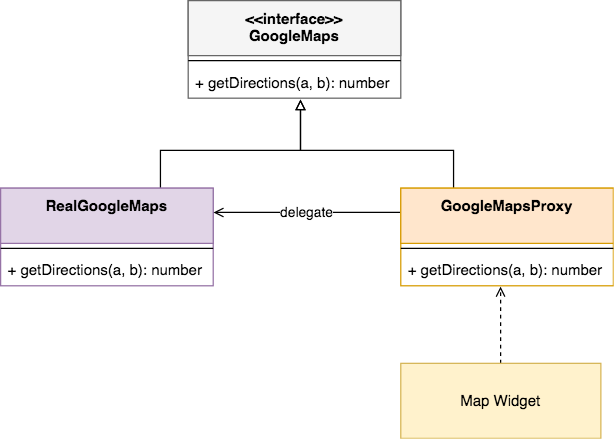
\includegraphics[width=1\columnwidth]{proxy} 
  \caption{Esempio di Proxy per GoogleMaps}
\end{figure}
             % Conclusioni

\appendix 
\blankpage
% !TEX encoding = UTF-8
% !TEX TS-program = pdflatex
% !TEX root = ../tesi.tex

%**************************************************************
\chapter{Tecnologie utilizzate}
%**************************************************************

\section{TypeScript}

\begin{figure}[H] 
  \centering 
  
\includegraphics[width=0.25\columnwidth]{ts} 
  \caption{TypeScript}
\end{figure}

TypeScript è un linguaggio di programmazione open-source sviluppato e mantenuto da Microsoft. La sua sintassi è un super-set di JavaScript, ovvero qualsiasi sintassi di quest'ultima è valida anche in TypeScript ma non vice-versa. TypeScript aggiunge difatti la possibilità di avere tipi statici. \\

TypeScript è progettato per lo sviluppo di grandi applicazioni e compila in JavaScript, per cui può essere usato sia per l'esecuzione lato client che server (Node.js). \\

Il linguaggio fornisce i tipi statici attraverso \textit{type annotations} che attivano il controllo dei tipi a tempo di compilazione. La scelta è tuttavia opzionale ed è possibile scrivere normale codice JavaScript senza tipi. \\

\begin{lstlisting}[language={[Sharp]C}]
function add(left: number, right: number): number {
  return left + right;
}
\end{lstlisting}

I tipi statici possono anche essere esportati dopo la compilazione in file di dichiarazione separati, in modo da fornire le informazioni sui tipi a chi deve utilizzare la libreria, la quale sarà già stata compilata in JavaScript. \\

Sia la libreria \textit{Stargate} che l'applicazione \textit{WorkWave Route Manager} sono scritte in TypeScript 3.0, rilasciato ad agosto 2018.

\section{React}

\begin{figure}[H] 
  \centering 
  
\includegraphics[width=0.25\columnwidth]{react} 
  \caption{React}
\end{figure}

\textbf{React} è una libreria JavaScript per la realizzazione di applicazioni web, in particolare per la creazione di interfacce utenti. È mantenuta e sviluppata da Facebook, sebbene abbia anche una forte community open-source. \\

La seguente classe è un componente UI React, che accetta una proprietà \texttt{greeting}. Il metodo \texttt{ReactDOM.render} si occupa invece di creare un'istanza di tale componente, passando ad esso \texttt{"Hello World!"} come valore di \texttt{greeting} e renderizzando il componente come figlio del nodo HTML avente id \texttt{"root"}. \\

\begin{lstlisting}[language={[Sharp]C}]
class Greeter extends React.Component { 
  render() { 
    return <h1>{this.props.greeting}</h1>
  } 
} 

ReactDOM.render(<Greeter greeting="Hello World!" />, document.getElementById('root'));
\end{lstlisting}

Di seguito sono invece elencate le caratteristiche principali di React, che hanno fortemente influenzato lo sviluppo moderno di web applications:

\begin{itemize}
  \item \textbf{One-way data binding con "props"}: tutte le informazioni esterne alla classe di cui ha bisogno il componente sono ricevute ed aggiornate tramite \texttt{props} dal componente genitore. Ciò assicura un flusso dei dati unidirezionale e predicibile. Inoltre le \texttt{props} sono da trattarsi come dati in sola lettura ed immutabili;
  \item \textbf{Componenti Stateful}: oltre alle \texttt{props}, i componenti possono avere uno stato interno utilizzabile internamente o passabile come \texttt{prop} ai figli.

  \vfill

    \begin{lstlisting}[language={[Sharp]C}]
class ParentComponent extends React.Component {
  state = { color: 'red' };

  render() {
    return (
      <ChildComponent color={this.state.color} />
    );
  }
}
    \end{lstlisting}

  \item \textbf{Virtual DOM}: il DOM è la rappresentazione in JavaScript della struttura HTML della pagina. React crea una propria rappresentazione virtuale del DOM dei componenti UI ed aggiorna efficientemente il DOM reale solo laddove necessario. Ciò consente al programmatore di descrivere il \texttt{render} dell'intera applicazione in base a \texttt{props} e \texttt{state}, mentre React si occupa delle effettive modifiche necessarie al DOM;
  \item \textbf{JSX}: è un'estensione della sintassi JavaScript per poter scrivere un codice simile all'HTML, ma dinamicamente in JavaScript, invece che come stringa statica.
\end{itemize}

React può essere usato come libreria di appoggio per lo sviluppo di applicazioni sia web che mobile e spesso è accompagnata da ulteriori librerie, quali \textit{Redux}, per la gestione dello stato, delle rotte o delle richieste server.

\section{Redux}

\begin{figure}[H] 
  \centering 
  
\includegraphics[width=0.25\columnwidth]{redux} 
  \caption{Redux}
\end{figure}

\textbf{Redux} è una libreria JavaScript per la gestione dello stato applicativo, che può essere visto come l'equivalente dello stato di un componente React ma relativa all'intera applicazione. La libreria implementa l'architettura \textit{Flux}, un'alternativa al popolare Model-View-Controller e che si avvicina più ad architetture ad eventi/messaggi. \\

In Redux, oggetti chiamati \textit{actions} hanno il compito di descrivere l'intenzione di modifica dello stato applicativo. Tale messaggio viene inviato allo \textit{Store}, il quale gestisce la modifica dello stato applicativo in base all'\textit{actions} e notifica la view (React) del cambiamento. Nessuna classe, ad eccezione dello \textit{Store}, ha la possibilità quindi di aggiornare lo stato applicativo, trattato come immutabile. \\

All'interno dello \textit{Store}, l'aggiornamento dello stato applicativo avviene attraverso i \textit{reducer}, funzioni pure aventi la firma \texttt{(State, Action) => State} e componibili tra di loro. \\

Si genera quindi un flusso unidirezionale, in cui la view riceve i dati e notifica di eventi tramite \textit{actions}. Quest'ultimi sono passati ai \textit{reducers} che producono un nuovo stato applicativo, passato dallo \textit{Store} nuovamente alla view.

\begin{figure}[H] 
  \centering 
  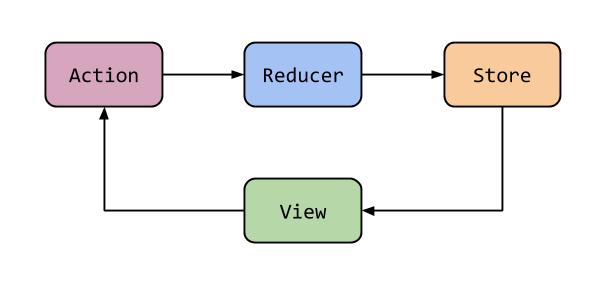
\includegraphics[width=0.75\columnwidth]{flux} 
  \caption{Flusso unidirezionale in Redux}
\end{figure}
             % Appendice A

%**************************************************************
% Materiale finale
%**************************************************************
\backmatter
\printglossaries
% !TEX encoding = UTF-8
% !TEX TS-program = pdflatex
% !TEX root = ../tesi.tex

%**************************************************************
% Bibliografia
%**************************************************************

\cleardoublepage

\begin{thebibliography}{9}
  \raggedright
  
  \bibitem{multiprocess} Chrome Multi-process architecture. URL: \url{https://www.chromium.org/developers/design-documents/multi-process-architecture}
  \bibitem{multiprocess-strategies} Chrome Multi-process strategies . URL: \url{https://www.chromium.org/developers/design-documents/process-models}
  \bibitem{noopener} About rel=noopener . URL: \url{https://mathiasbynens.github.io/rel-noopener/}
  \bibitem{deep-copy} Deep-copying in JavaScript . URL: \url{https://dassur.ma/things/deep-copy/}
  \bibitem{broadcastchannel} BroadcastChannel API . URL: \url{https://developer.mozilla.org/en-US/docs/Web/API/Broadcast_Channel_API}
  \bibitem{crosstab} Crosstab. \textit{A utility library for cross-tab communication using localStorage}. URL:  \url{https://github.com/tejacques/crosstab}
  \bibitem{webworkers} Using Web Workers . URL: \url{https://developer.mozilla.org/en-US/docs/Web/API/Web_Workers_API/Using_web_workers}
  \bibitem{rpc} Remote Procedure Call . URL: \url{https://en.wikipedia.org/wiki/Remote_procedure_call}
\end{thebibliography}

\end{document}
